\documentclass[10pt]{IEEEtran}
%\documentclass[10pt]{article}
\usepackage[spanish]{babel} % Definir el idioma del documento
\usepackage[letterpaper,top = 2cm, bottom = 2cm, left = 2cm, right = 2cm, marginparwidth = 1.75cm]{geometry} % Especificar los márgenes según la norma
\usepackage{pdfpages} % Añadir PDFs y que te cuente las páginas para el documento
\usepackage{subfiles} % Tener subdocumentos (hay más opciones)
\usepackage{tableof} % Se utiliza para los indices de los subdocumentos
\usepackage{float} % Para usar lo de 'H'
\usepackage{fancyhdr}
\usepackage{comment}
\usepackage{biblatex} % Paquete para manejar citas y bibliografía
\usepackage{amsmath}
\usepackage{lipsum}
\usepackage{multirow}
\usepackage[font=footnotesize]{caption}

\addbibresource{bibliografia.bib} % Cargar el archivo .bib

\def\TituloProyecto{Puente de Cody Docks}
\def\Autor{Mercedes Román Ruiz}
\def\Asignatura{Máquinas Hidráulicas y Eólicas}
\def\Curso{2024 - 25}
\def\Fecha{23 Mayo 2025}

\begin{document}
\sloppy 
\renewcommand{\baselinestretch}{1}
\renewcommand{\listtablename}{Índice de tablas}
\renewcommand{\tablename}{Tabla}
\setlength{\parindent}{0pt} % Sangría al comienzo del párrafo
\setlength{\parskip}{10pt} % Espacio entre dos párrafos
\renewcommand\thesection{\arabic{section}}
\renewcommand{\baselinestretch}{1.5}

\begin{titlepage}
    \centering
    
\includegraphics[width=0.5\linewidth]{Imagenes/Logo UPM.png} \par
    \vspace{1cm}
    {\bfseries\LARGE Escuela Técnica Superior de Ingenieros Industriales \par}
    \vspace{0.5cm}
    {\scshape\Large Máster en Ingeniería Industrial \par}
    \vspace{1.5cm}
    {\scshape\Huge \Asignatura \par}
    \vspace{3 cm}
    {\Huge \textbf{GRUPO L} \par}
    \vfill
    {\Large \Fecha \par}
\end{titlepage}

% --------------------------------------------------------------------------------------------
% El uso de negrita debería ser ocasional, y la cursiva debe utilizarse para términos en otro idioma. El texto debe estar ''justificado'', esto es, el párrafo cubrirá todo el ancho de la columna salvo punto final. El espaciado entre líneas está fijado a 1,0, mientras que el espaciado entre párrafos es el fijado por defecto. No se hará uso de sangría al inicio de un párrafo pues éstos quedan identificados con el espaciado entre párrafos.
% --------------------------------------------------------------------------------------------

% Cada grupo elabora un único informe, para lo que puede seguir el formato de la plantilla adjunta, o realizarlo en LaTeX con una plantilla propia (opción recomendada).

% El informe ha de constar de título general del informe, nombre de la asignatura y código, inicial(es) y apellidos de *todos* los miembros del grupo, correo electrónico, número de matrícula, resumen, palabras claves, introducción, desarrollo, conclusiones y bibliografía.

% El informe debe indicar expresamente los miembros que actúan como "coordinadores del grupo", responsables de supervisar la elaboración y entrega del informe mediante un reparto de tareas adecuado entre todos los miembros

% La extensión máxima del informe es 30 páginas.

\onecolumn

\begin{table}[h!]
    \centering
    \caption{Miembros del grupo (los coordinadores se indican en \textbf{negrita}).}
    \label{tab: Miembros}
    \begin{tabular}{|c|c|c|c|}
        \hline
        Apellidos & Nombre & Número de Matrícula & Correo Electrónico \\
        \hline
        Arvilla Maldonado & Borja & 20027 & borja.arvilla@alumnos.upm.es \\
        Bacaicoa Morrás & Clara & M24113 & clara.bacaicoa@alumnos.upm.es \\
        Carrillo Migoya & Aitana & 20052 & aitana.carrillo@alumnos.upm.es \\
        Diego Fernandez & Paula De & 19087 & paula.dediegof@alumnos.upm.es \\
        Durán Haro & Marina & 20100 & marina.duran@alumnos.upm.es \\
        \textbf{García Aguilera} & \textbf{Juan} & \textbf{20127} & \textbf{juan.garcia.aguilera @alumnos.upm.es} \\
        Gómiz Villamor & Carlos & 19160 & c.gomiz@alumnos.upm.es \\
        González Muruaga & Ariane & M24129 & ariane.gonzalez@alumnos.upm.es \\
        Limón López & Marta Victoria & 20732 & m.limon@alumnos.upm.es \\
        Marañón Heras & Pablo & 19222 & pablo.marheras@alumnos.upm.es \\
        Montes Núñez & Paloma Henar & 20742 & palomahenar.mnunez@alumnos.upm.es \\
        Moreno Serrano & Pablo Miguel & 24012 & pablo.moreno.serrano@alumnos.upm.es \\
        Moya Alonso & Inés & M23275 & in.moya@alumnos.upm.es \\
        Pérez Costa & Álvaro & 24076 & a.pcosta@alumnos.upm.es \\
        \textbf{Portero Moreno} & \textbf{Jorge} & \textbf{19036} & \textbf{jorge.portero.moreno@alumnos.upm.es} \\
        \textbf{Roman Ruiz} & \textbf{Mercedes} & \textbf{M24210} & \textbf{mercedes.roman@alumnos.upm.es} \\
        Santón López & Blanca & 20322 & blanca.santon@alumnos.upm.es \\
        Sanz Bravo & Nieves & 19345 & nieves.sbravo@alumnos.upm.es \\
        Tiemblo Martín-Calderín & José Ramon & 19358 & jr.tiemblo@alumnos.upm.es \\
        \hline
    \end{tabular}
\end{table}

\pagebreak

\section*{Resumen}

El presente informe recoge el análisis experimental del comportamiento de tres tipos de máquinas hidráulicas y eólicas: bombas centrífugas, turbinas hidráulicas tipo Pelton y aeroturbinas de eje horizontal. A través de los ensayos realizados en laboratorio, se han obtenido datos que permiten estudiar las curvas características de funcionamiento de cada máquina, así como validar las leyes de semejanza aplicables.

En el caso de las bombas hidráulicas, se han ensayado configuraciones en operación individual, en serie y en paralelo, con distintos regímenes de giro. Se han representado las curvas $\Delta P - Q$ tanto en forma dimensional como adimensional, y se ha comparado el comportamiento real con las predicciones teóricas derivadas del análisis dimensional.

Para la turbina Pelton, se ha analizado su funcionamiento a distintos caudales manteniendo constante el salto neto, obteniendo curvas de par, potencia y rendimiento en función de la velocidad de giro. Asimismo, se ha calculado la velocidad específica adimensional $\omega_s$.

Finalmente, en la aeroturbina se ha estudiado el efecto del ángulo de paso $\beta$ sobre el coeficiente de potencia $C_P$ y la velocidad específica $\lambda$, obteniendo curvas $C_P - \lambda$ para distintos valores de $\beta$ y velocidades del viento. Se ha observado la tendencia esperada conforme a la teoría de funcionamiento de estas máquinas.


% Debería incluirse un resumen al inicio del informe, que se indica cuál es el objetivo de cada práctica, la metodología seguida y los resultados y las conclusiones más significativas. En el resumen no deben aparecer referencias.

\section*{Nomenclatura}
\begin{tabular}{ll}
$Q$ & Caudal volumétrico [m$^3$/s] \\
$\Delta P$ & Incremento de presión [Pa] \\
$H$ & Altura manométrica [m] \\
$P$, $W$ & Potencia [W] \\
$\eta$ & Rendimiento de la máquina [-] \\
$\omega$ & Velocidad angular [rad/s] \\
$n$ & Velocidad de giro [rpm] \\
$T$ & Par [Nm] \\
$C_P$ & Coeficiente de potencia [-] \\
$C_v$ & Coeficiente de velocidad [-] \\
$C_q$ & Coeficiente de caudal [-] \\
$\lambda$ & Velocidad específica adimensional [-] \\
$\omega_s$ & Velocidad específica adimensional [-] \\
$n_s$ & Velocidad específica dimensional (número de Camerer) \\
$\beta$ & Ángulo de paso de las palas [º] \\
$\rho$ & Densidad del fluido [kg/m$^3$] \\
$\mu$ & Viscosidad dinámica del fluido [Pa·s] \\
$v$ & Velocidad del viento o del chorro [m/s] \\
$I$ & Intensidad de corriente [mA] \\
$U$ & Tensión [V] \\
$D$ & Diámetro del rodete o de las palas [m] \\
\end{tabular}


% Indíquese cinco palabras clave que haya extraído del trabajo realizado y que considere que represental al informe redactado.

\newpage
\twocolumn
{\LARGE Bombas Hidráulicas \par}
\setcounter{section}{0}
\setcounter{subsection}{0}
\setcounter{subsubsection}{0}

\section{Introducción}

Las máquinas hidráulicas, como las bombas y turbinas, son dispositivos esenciales en ingeniería, ya que convierten la energía hidráulica en trabajo útil. En este caso, una bomba centrífuga es utilizada para aumentar presión de un fluido mediante energía externa, destacando parámetros como caudal, presión y eficiencia operativa. En esta práctica se estudia una bomba centrífuga con configuraciones variables, permitiendo su funcionamiento en serie, paralelo o de forma individual:

\begin{itemize}
  \item En serie: incrementa la presión total al pasar el fluido de una bomba a otra.
  \item En paralelo: aumenta el caudal al dividir el flujo entre las bombas.
\end{itemize}

El marco teórico se basa en el Teorema de $\pi$-Buckingham, que simplifica los problemas físicos mediante variables adimensionales, permitiendo aplicar relaciones de semejanza para predecir el comportamiento de las bombas bajo diferentes condiciones operativas.

\subsection{Objetivos de la práctica}
Los objetivos principales de esta práctica son:
\begin{enumerate}
  \item Verificar la validez de la teoría de semejanza en bombas centrífugas, analizando las curvas características $\Delta P - Q$ obtenidas por distintas velocidades de giro ($73\%$ y $50\%$ de la velocidad nominal).
  \item Estudiar las variaciones en el rendimiento hidráulico de las bombas al operar en configuraciones individuales, en serie y en paralelo, evaluando el impacto en el caudal y presión. 
\end{enumerate}

\section{Descripción del equipo de prácticas y metodología}

El banco de ensayos utilizado en esta práctica está diseñado para analizar el comportamiento y rendimiento de bombas centrífugas bajo diferentes configuraciones. Este sistema está compuesto por varios elementos clave que permiten realizar mediciones precisas.

En primer lugar, el banco incluye dos bombas centrífugas con características diferenciadas. La bomba 1 tiene un régimen de giro ajustable, alcanzando una velocidad máxima de 1.800 rpm. Este control variable se logra mediante un regulador integrado, que facilita el análisis del comportamiento hidráulico bajo diferentes velocidades de operación. La bomba 2, por su parte, opera a una velocidad fija nominal, proporcionando un punto de referencia constante para las comparaciones entre configuraciones.

El sistema de tuberías y válvulas que acompaña al banco de ensayos permite alternar entre configuraciones de operación individual, en serie y en paralelo. Las válvulas de control, estratégicamente colocadas, hacen posible ajustar el flujo desde valores mínimos hasta el caudal máximo admisible. Esto permite estudiar cómo varían el caudal y la presión generados por las bombas según las condiciones impuestas.

El flujo de agua es suministrado por un depósito de alimentación, que proporciona un suministro continuo y estable durante las mediciones.

Finalmente, el banco está equipado con sensores avanzados conectados a un sistema de monitoreo digital mediante el software Armfield. Estos sensores registran parámetros críticos como el caudal y la presión. Con el software Armfield se puede controlar los parámetros operativos, registrar los datos experimentales y realizar cálculos relacionados con la altura total, la potencia y la eficiencia hidráulica.

\subsection{Metodología}
En cada configuración de las bombas (individual, serie y paralelo), el procedimiento incluye:
\begin{itemize}
  \item Alimentar el sistema con agua desde el depósito de alimentación.
  \item Regular el flujo mediante las válvulas principales, variando el caudal progresivamente desde el mínimo hasta el máximo permitido.
  \item Registrar las lecturas de presión y caudal en diferentes puntos de operación, utilizando el software de monitoreo.
  \item Analizar las curvas características $\Delta P - Q$ para cada configuración y comparar los resultados experimentales con las prediciones teóricas basadas en las leyes de semejanza.
\end{itemize}

\subsection{Características del bando de ensayos FM51}
El banco de ensayos es un sistema de precisión diseñado para evaluar el rendimiento de bombas hidráulicas. Sus especificaciones incluyen:
\begin{itemize}
  \item Caudal máximo: $2.2\ L/s$ (en paralelo)
  \item Altura máxima: $6\ m$ (una sola bomba) $12\ m$ (en serie)
  \item Velocidad máxima de la bomba: $1800\ rpm$ (bomba 1) y $1500\ rpm$ (bomba 2 nominal)
  \item Potencia del motor: $180\ W$
\end{itemize}

\section{Resultados}

\subsection{Bomba en operación individual}

A continuación, se presentan los resultados obtenidos en el estudio del funcionamiento de una bomba centrífuga en operación individual. Se han realizado ensayos a dos velocidades de giro distintas - el $73\%$ y el $50\%$ de la velocidad nominal - con el objetivo de comprobar si se cumple la teoría de semejanza.

Para cada velocidad, se recogen los valores de caudal ($Q$) y salto de presión ($\Delta P$), a partir de los cuales se construyen las curvas características $\Delta P - Q$. Además, se incluyen en la misma gráfica los valores teóricos correspondientes a la segunda velocidad, obtenidos mediante las relaciones de semejanza

Por último, se representan los resultados de forma adimensional mediante los coeficientes $\frac{\Delta P}{\rho \omega^2 D^2}$ y $\frac{Q}{\omega D^3}$, lo que permite comparar el comportamiento de la bomba en condiciones distintas y verificar si los datos experimentales siguen la tendencia prevista por la teoría. 

\begin{figure*}[ht!]
  \centering
  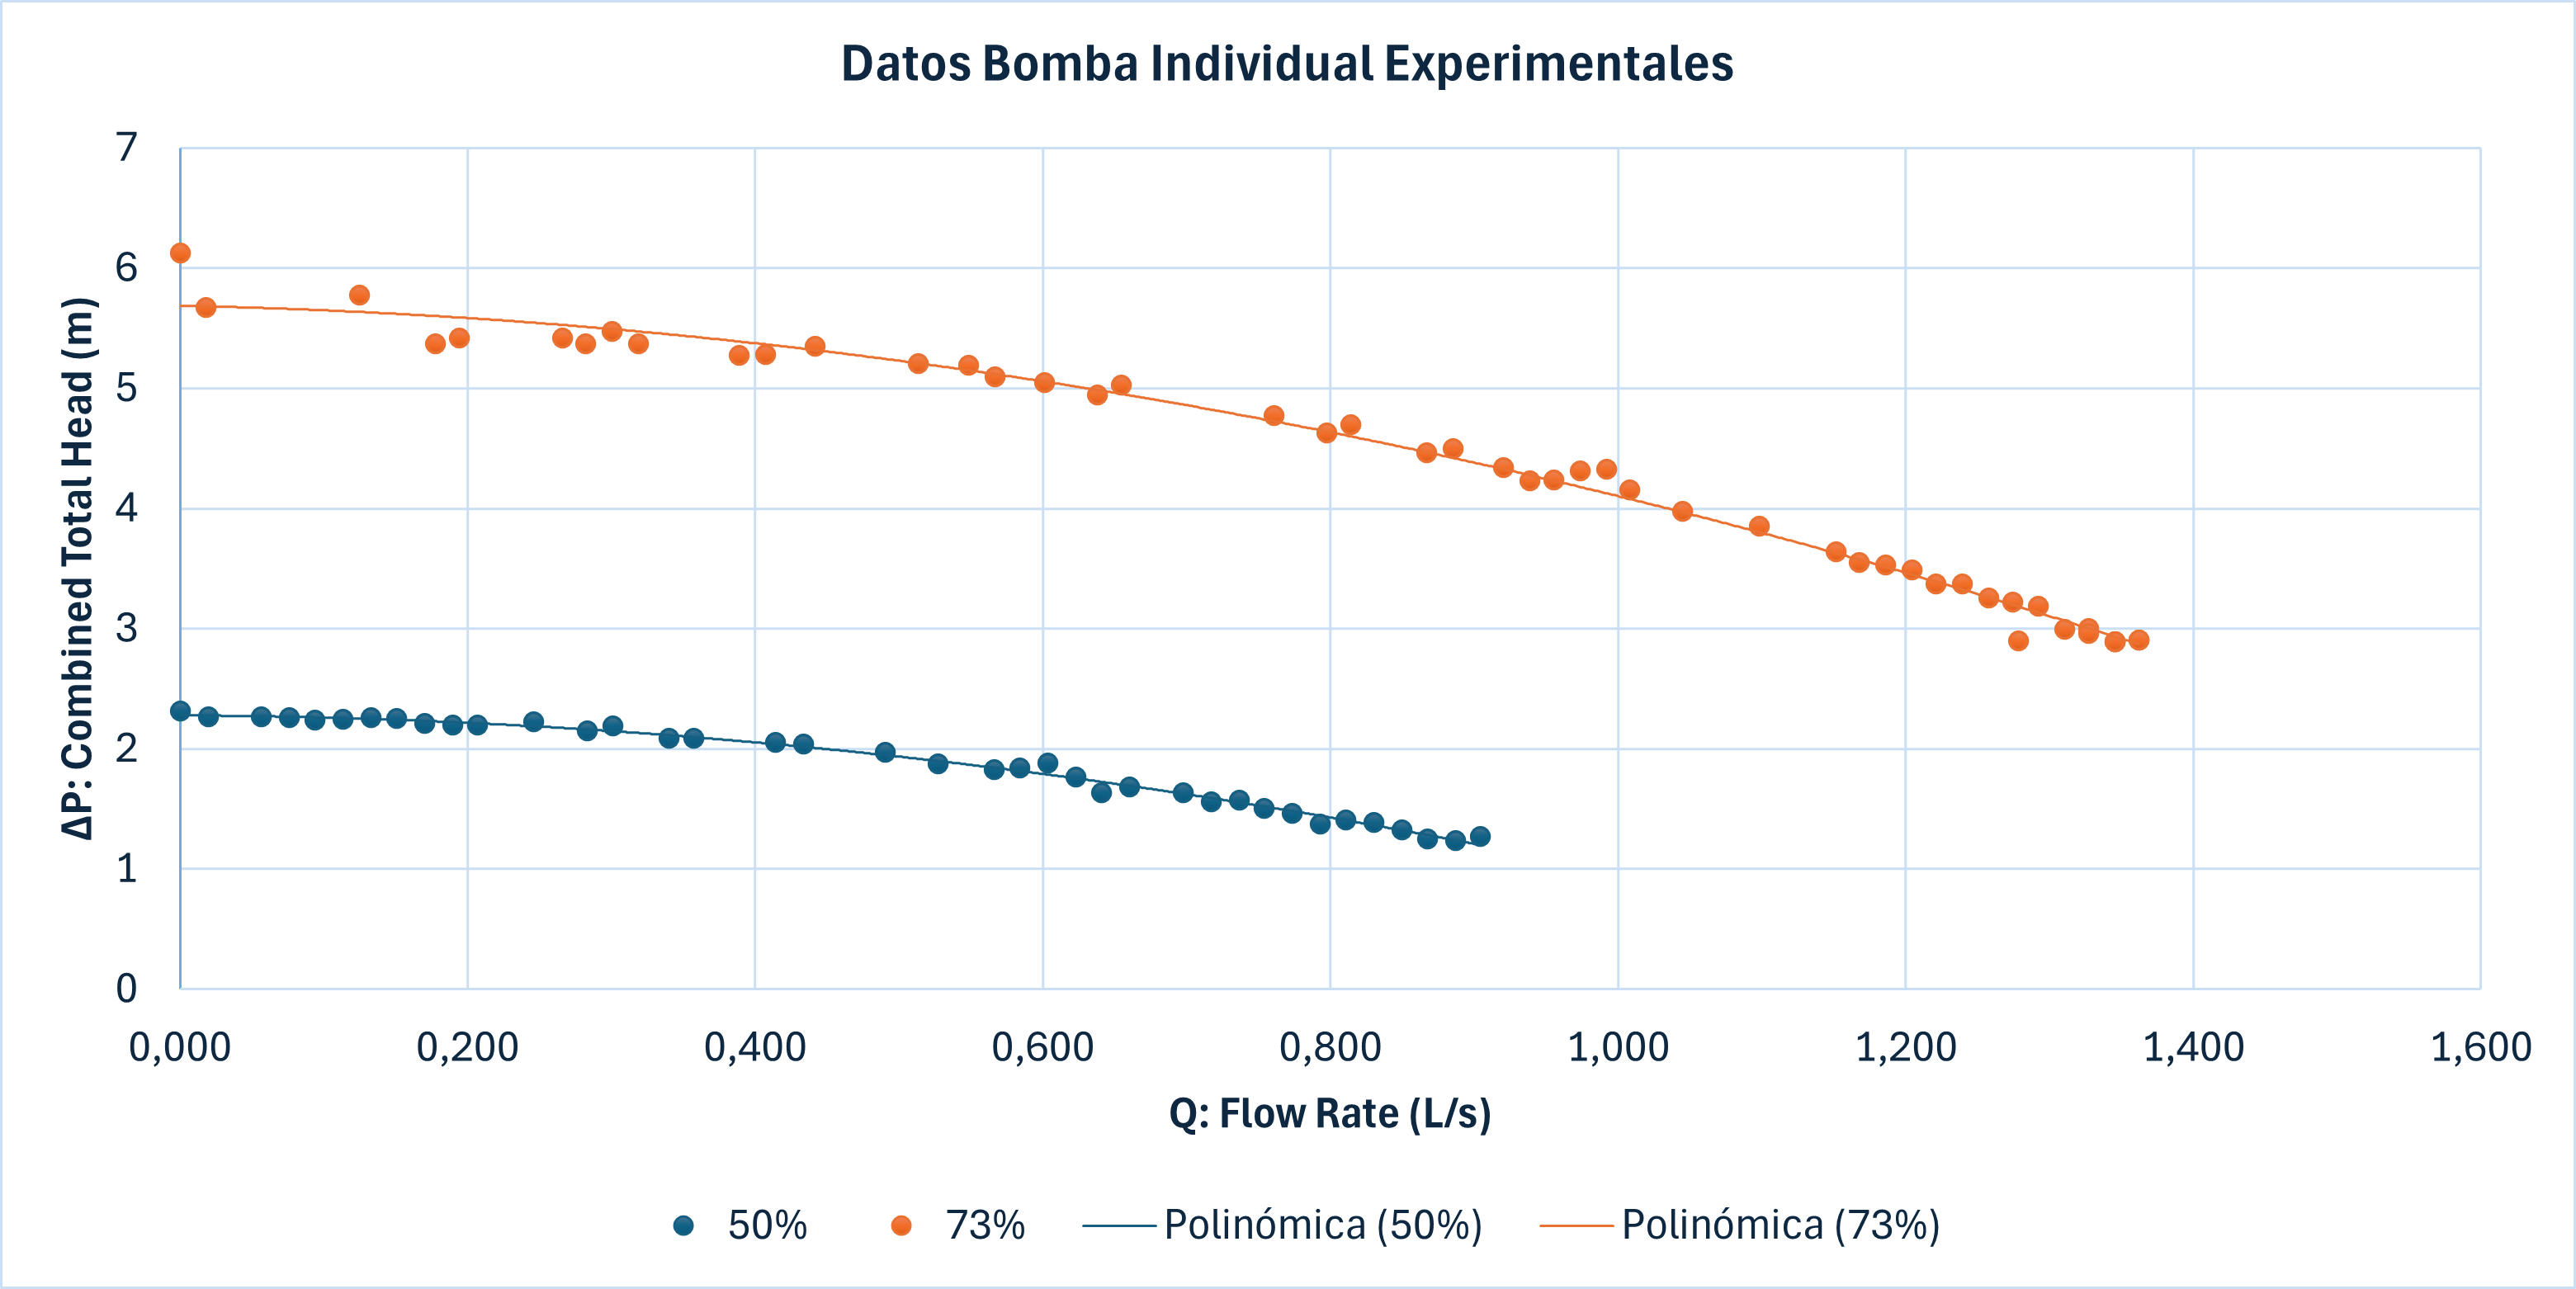
\includegraphics[width= 0.75 \textwidth]{Imagenes/Datos Bomba Individual Experimentales.png}
  \caption{Curvas características $\Delta P - Q$ obtenidas experimentalmente para una bomba centrífuga en operación individual, a dos velocidades de giro: $73\%$ y $50\%$ de la velocidad nominal.} 
  \label{fig: Datos Bomba Individual Experimentales}
\end{figure*}

La Figura \ref{fig: Datos Bomba Individual Experimentales} muestra las curvas características obtenidas experimentalmente para la bomba en operación individual a dos velocidades distintas. Tal como se observa, al disminuir la velocidad de giro desde el $73\%$ al $50\%$ de la velocidad nominal, se reduce tanto el caudal máximo alcanzado como el salto de presión generado por la bomba. Además, la forma general de las curvas se mantiene coherente con el comportamiento típico de una bomba centrífuga, presentando una caída progresiva de presión conforme aumenta el caudal. 

Estos resultados confirman que el rendimiento hidráulico de la bomba se va directamente afectado por la velocidad de funcionamiento. 

\begin{figure*}[ht!]
  \centering
  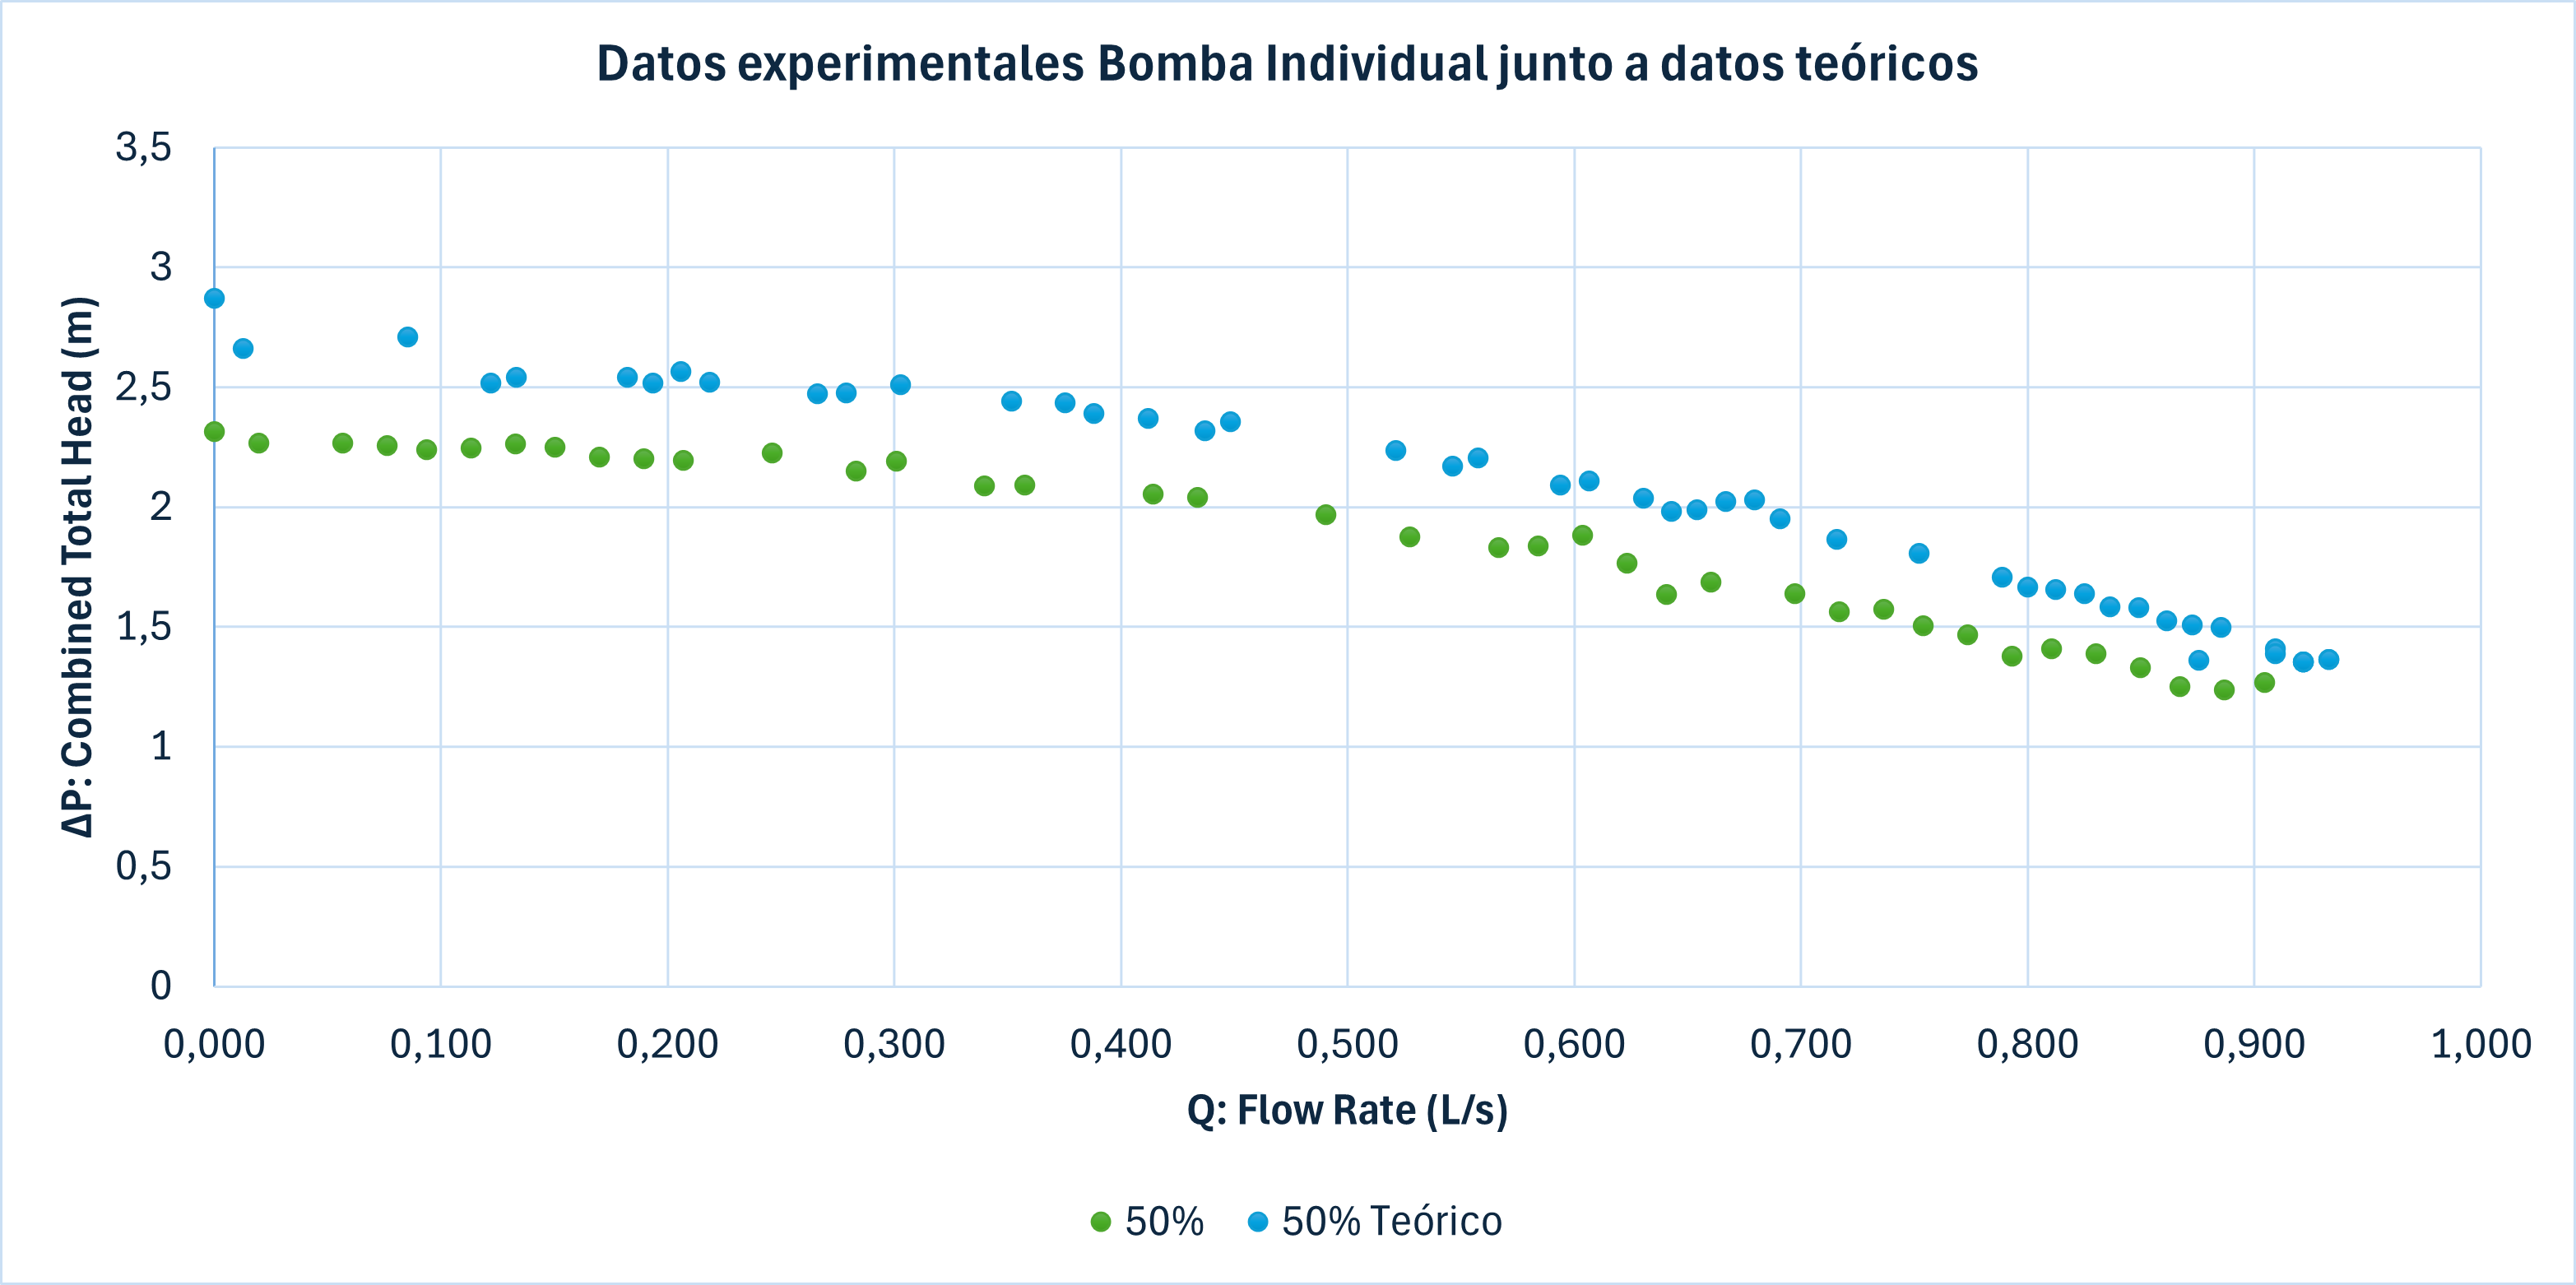
\includegraphics[width= 0.75 \textwidth]{Imagenes/Datos experimentales Bomba Individual junto a datos teóricos.png}
  \caption{Comparación entre los datos experimentales y los valores teóricos por semejanza para la bomba en operación individual al $50\%$ de la velocidad nominal.} 
  \label{fig: Datos experimentales Bomba Individual junto a datos teóricos}
\end{figure*}

En la Figura \ref{fig: Datos experimentales Bomba Individual junto a datos teóricos} se comparan los datos experimentales obtenidos a una velocidad del $50\%$ de la nominal ($1800rpm$) con los valores teóricos estimados mediante las leyes de semejanza, a partir de los resultados experimentales registrados al $73\%$. En general, ambas curvas presentan una forma similar y siguen la misma tendencia descendente de salto de presión con el aumento del caudal.

La diferencia entre ambas curvas se mantiene relativamente constante, aunque se aprecia una mayor proximidad en la zona de caudales elevados, a partir de aproximadamente 0,6 L/s. En ese intervalo, las diferencias entre ambas curvas se reducen, lo que sugiere que el comportamiento de la bomba bajo condiciones reales se ajuste mejor a las predicciones teóricas en ese rango de operación. 

\begingroup
\captionsetup{justification=centering}
\begin{figure*}[ht!]
  \centering
  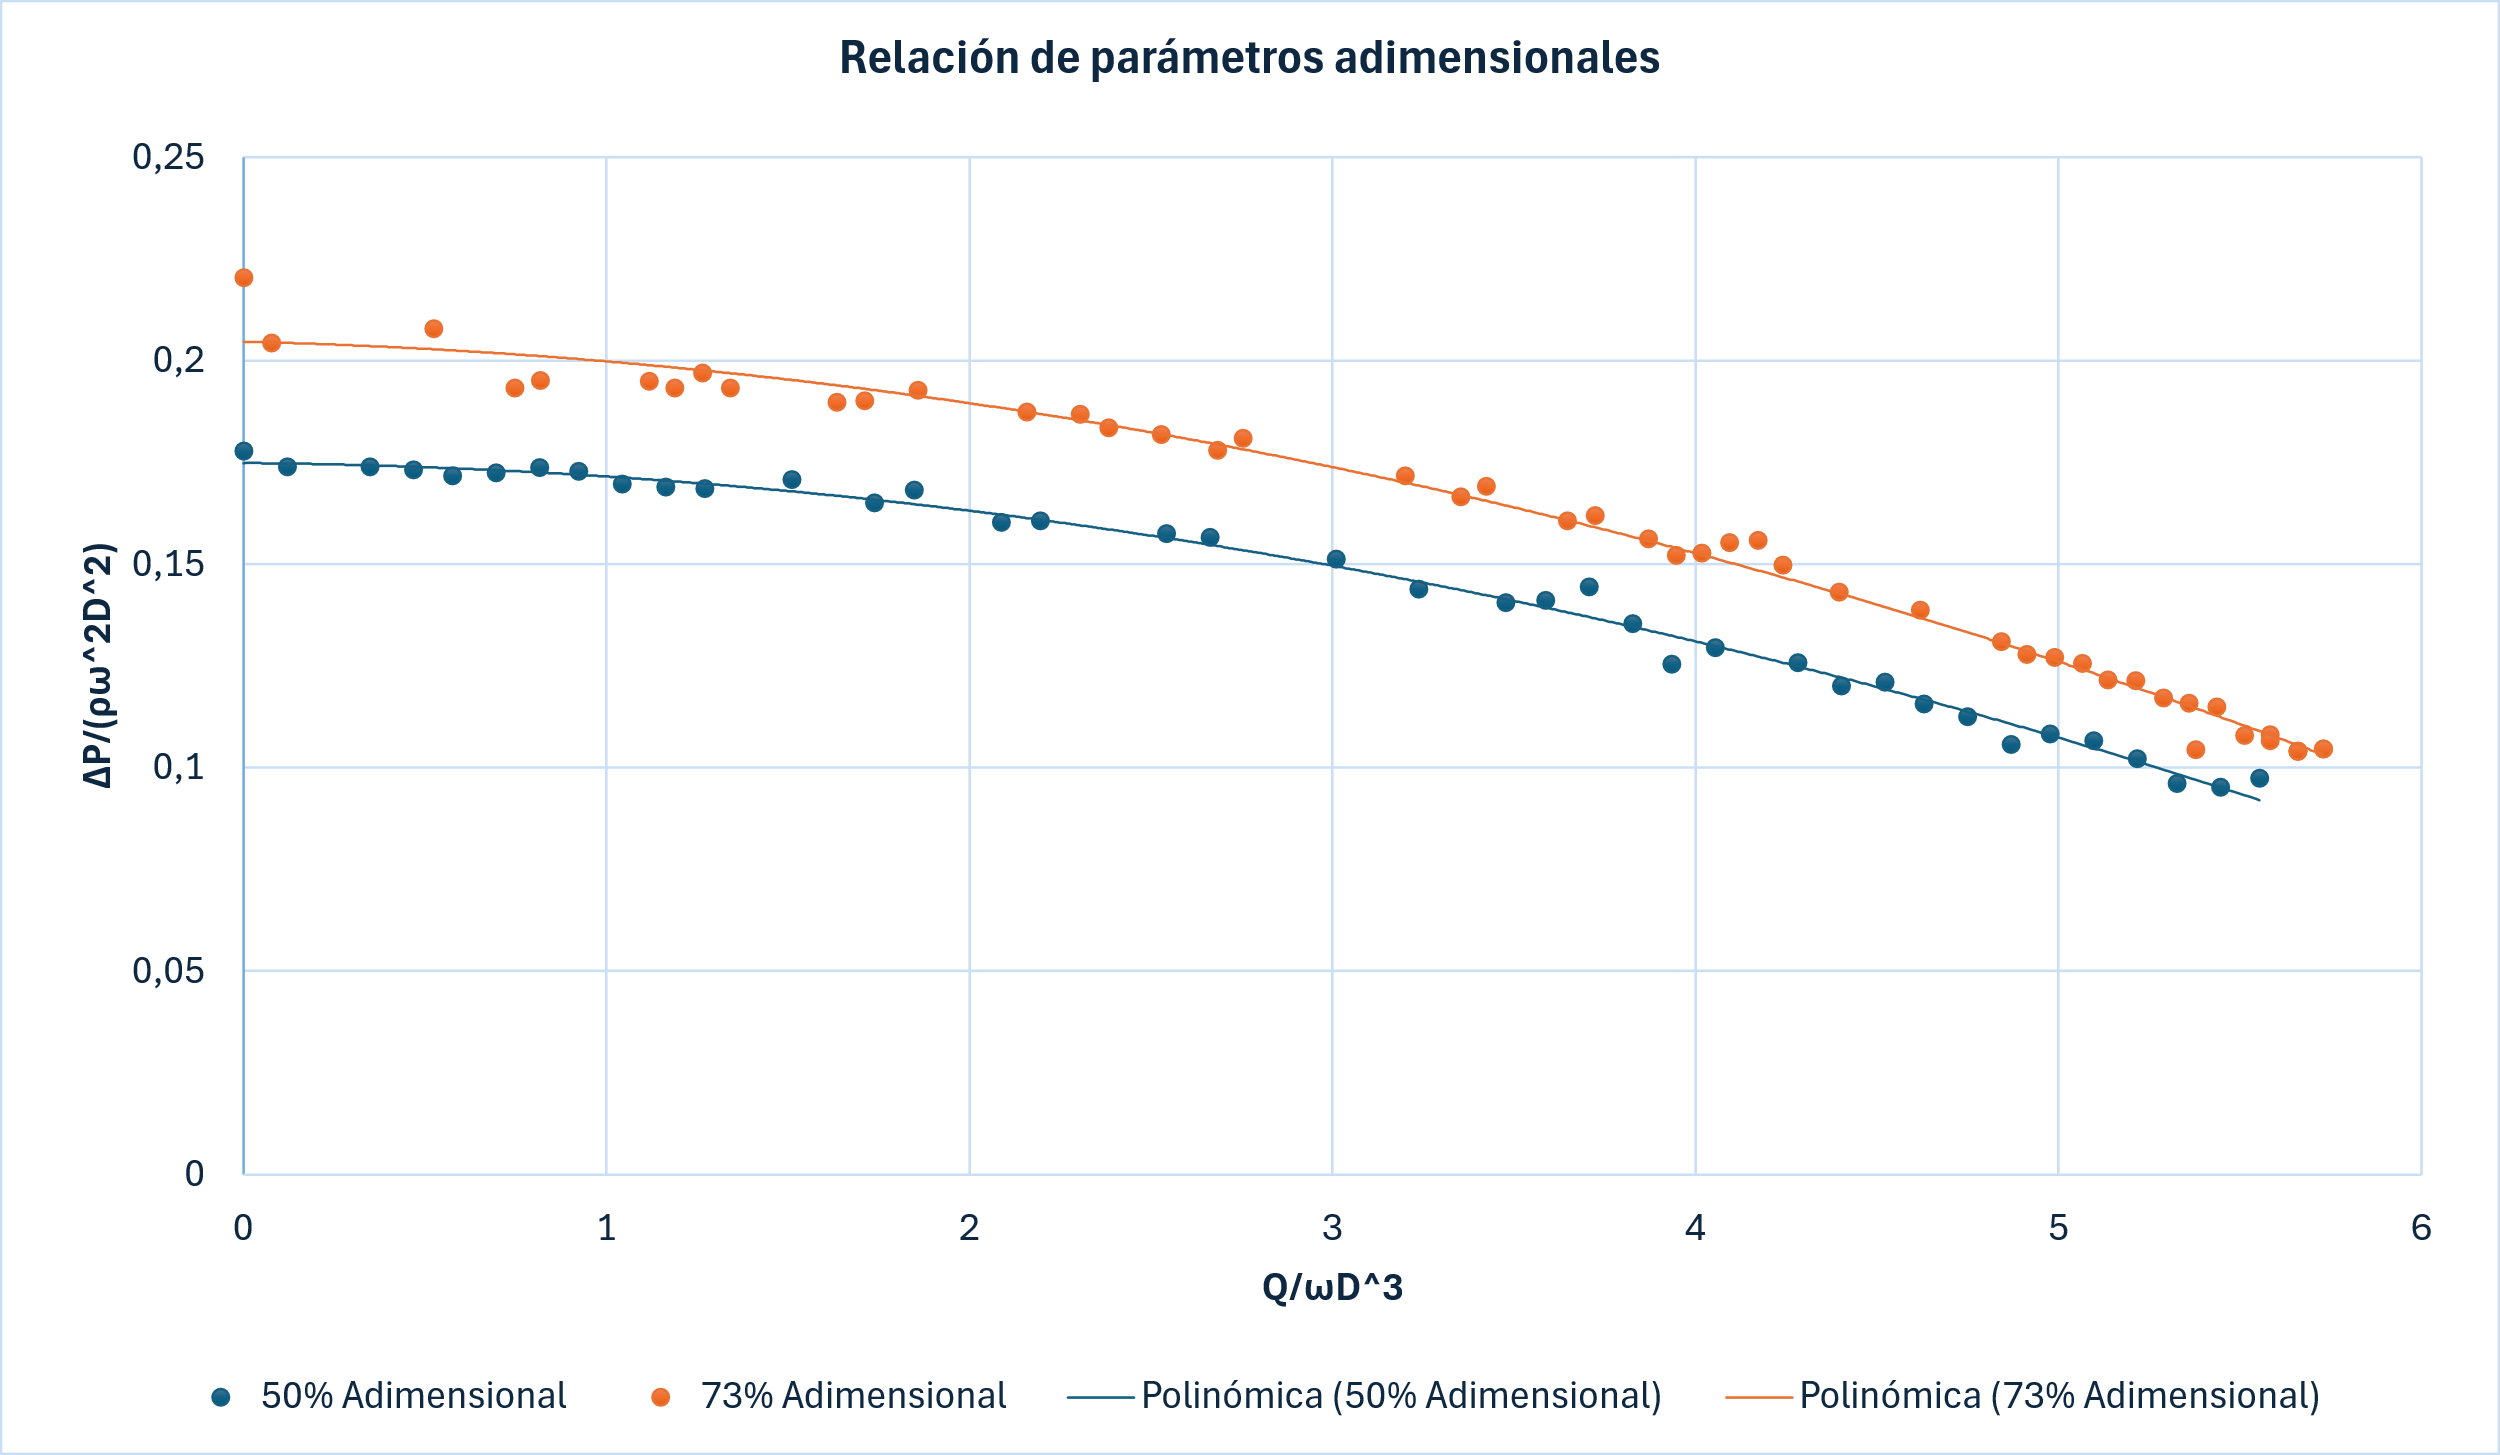
\includegraphics[width= 0.75 \textwidth]{Imagenes/Relacion de parametros adimensionales.png}
  \caption{Representación adimensional de la bomba en operación individual a dos velocidades ($73\%$ y $50\%$ de la velocidad nominal)} 
  \label{fig: Relacion de parametros adimensionales}
\end{figure*}
\endgroup

La Figura \ref{fig: Relacion de parametros adimensionales} muestra la relación entre los coeficientes adimensionales de presión y caudal para la bomba en operación individual a dos velocidades distintas. Aunque ambas curvas mantienen una tendencia coherente, no se produce una superposición exacta, lo cual indica que las condiciones de semejanza no se cumplen perfectamente. Sin embargo, la gráfica resulta útil para visualizar cómo varían los coeficientes sin depender de las unidades específicas, y destaca que el comportamiento global de la bomba sigue un patrón similar entre ambas condiciones de ensayo. 

\subsubsection{Conclusiones}

Los resultados confirman que las leyes de semejanza son herramientas útiles para analizar el comportamiento de una bomba centrífuga bajo diferentes condiciones operativas, aunque presentan limitaciones en su aplicación exacta.

\subsection{Bombas en operación en serie}
En este apartado se estudia la configuración de bombas en serie, en el que el fluido circula desde la bomba 1 hasta la bomba 2. En primer lugar se examina el efecto de tener una bomba frente a dos en serie, girando en ambas disposiciones al $73\%$ de su velocidad máxima. Posteriormente se hace la comparación de dos bombas en serie con distinto régimen de giro, siendo una al $50\%$ del máximo y otra al $73\%$. Estas dos situaciones se estudiaran representando las curvas características  dimensionales de salto de presión ($\Delta P$) en metros ($m$) frente a caudal ($Q$) en litros por segundo ($L/s$).

\subsubsection{Comparación: $73\%$ individual vs $73\%$ serie}

\begin{figure*}[ht!]
  \centering
  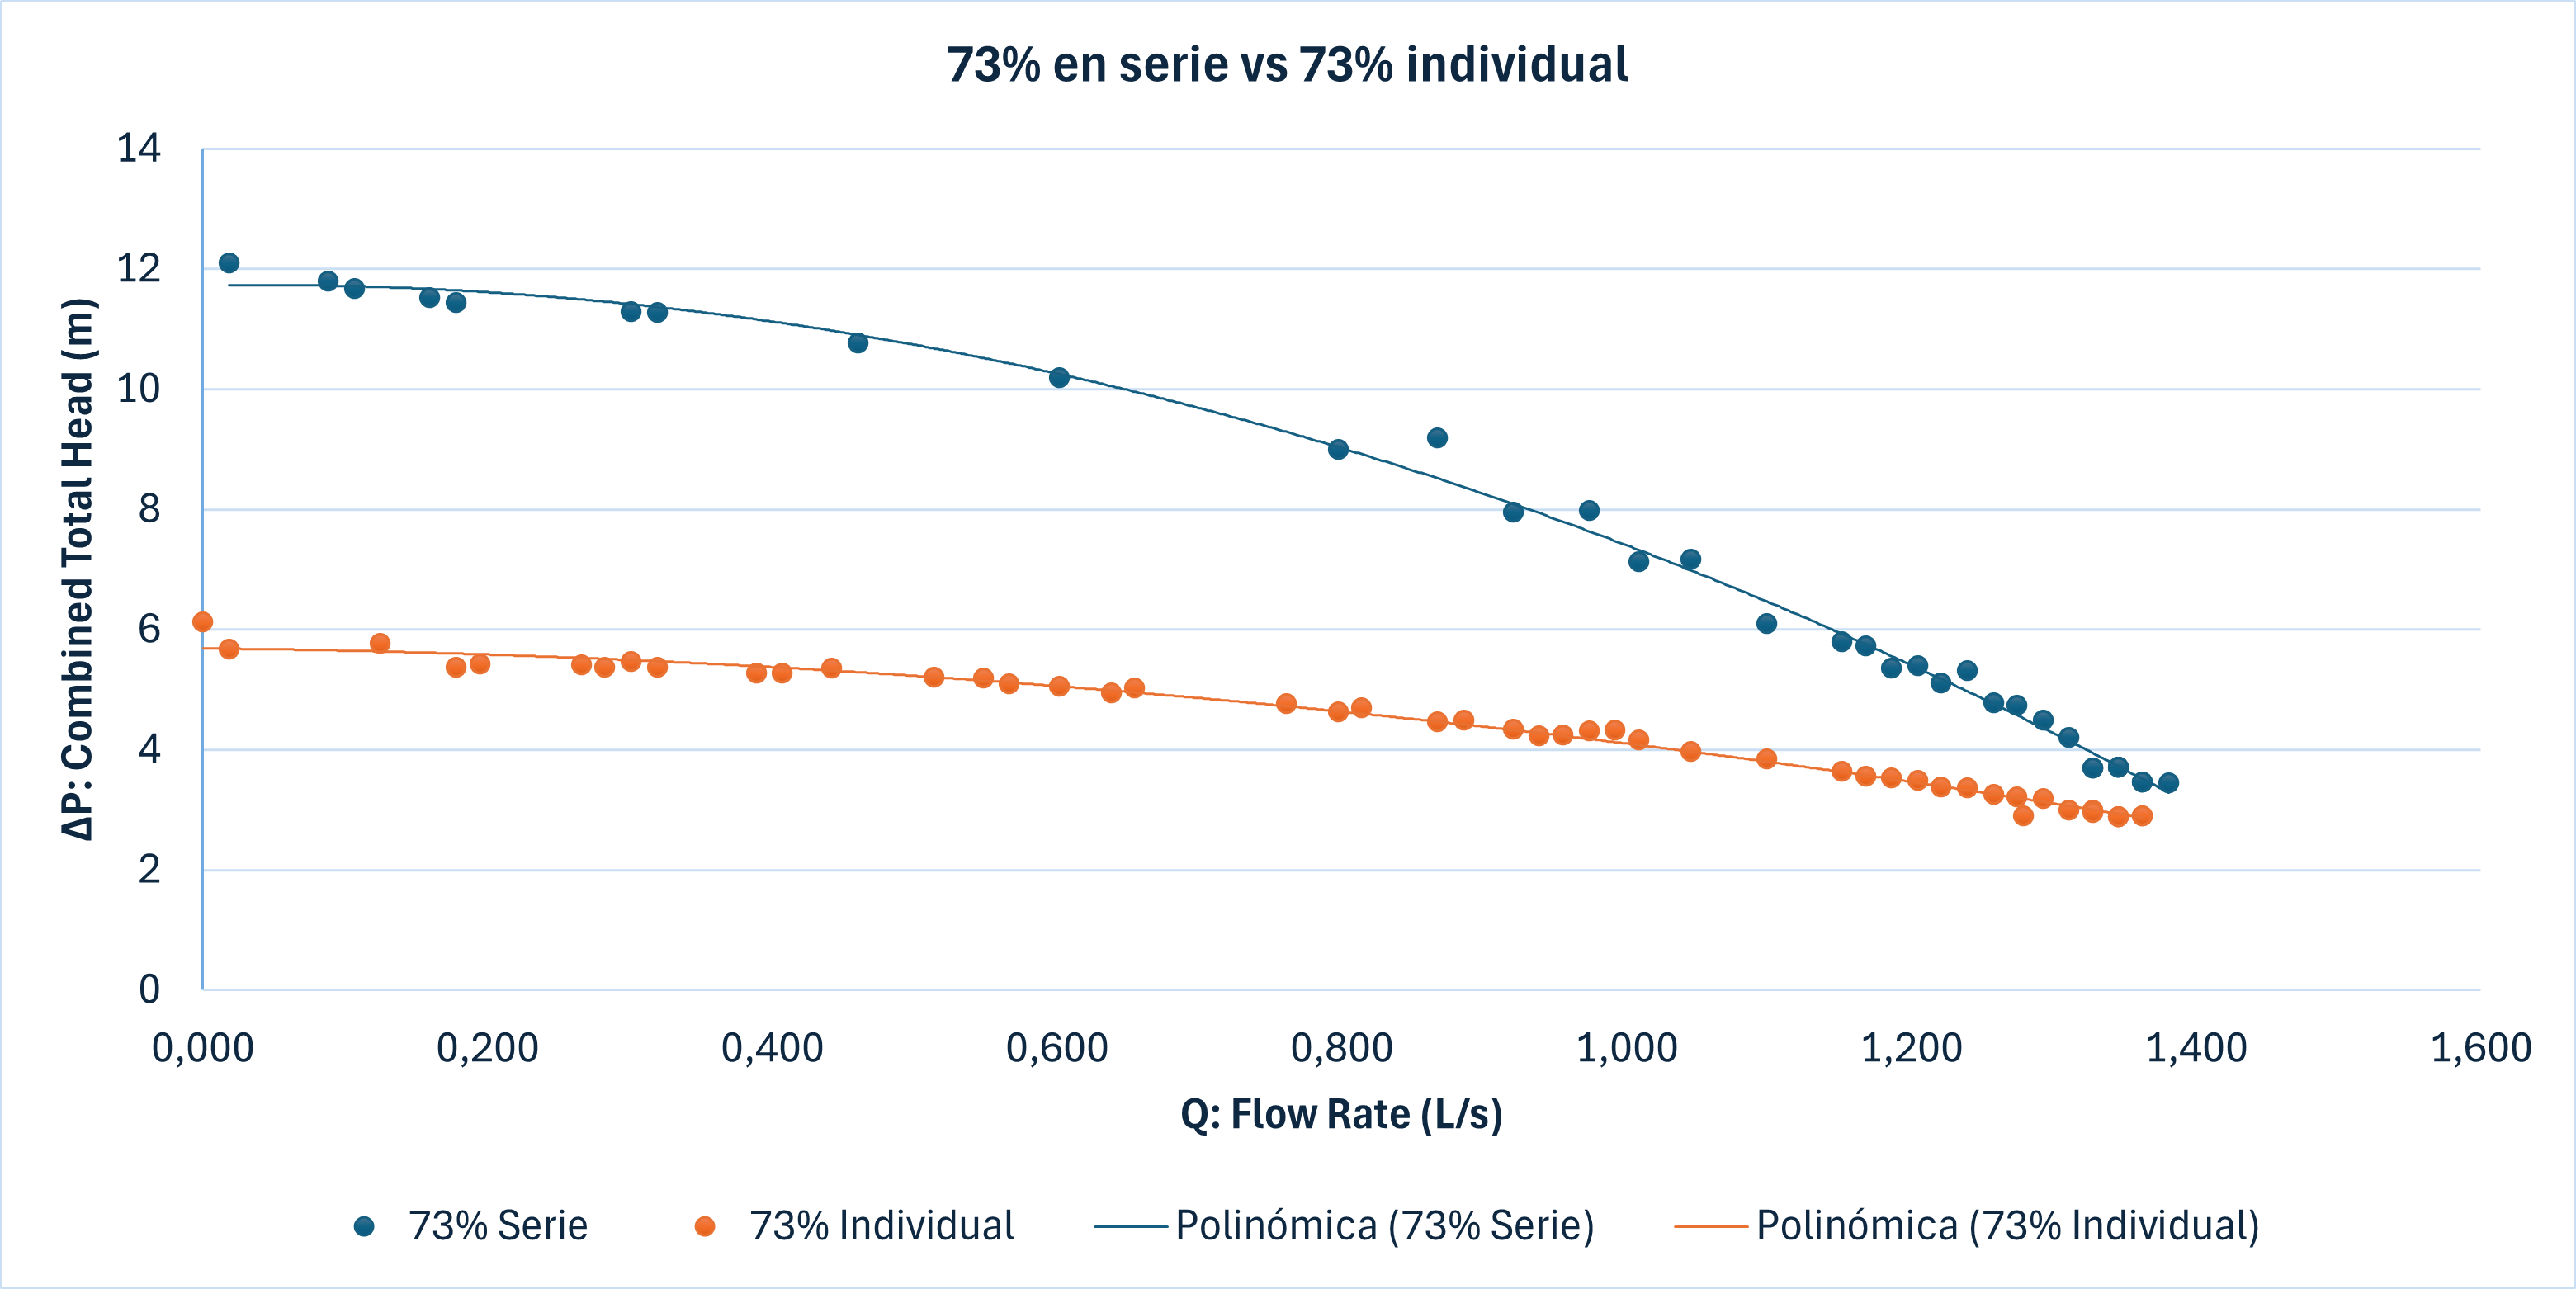
\includegraphics[width= 0.75 \textwidth]{Imagenes/BombasSerie Figura 1.png}
  \caption{Comparación de curvas características dimensionales de una bomba y una configuración en serie, ambas al $73\%$ de su velocidad de giro máxima.} 
  \label{fig: BombasSerie Figura 1}
\end{figure*}

De acuerdo con la teoría, el objetivo de utilizar la disposición en serie es conseguir una altura mayor para un mismo caudal. En la Figura \ref{fig: BombasSerie Figura 1}, donde se representa en el eje de abscisas el caudal y en el de ordenadas la altura, se puede comprobar experimentalmente que para caudales pequeños la altura de la configuración en serie es mucho mayor que la que proporciona una sola bomba, siendo esta la suma de la que proporcionarían las dos bombas por separado. Sin embargo, si nos desplazamos a caudales mayores este argumento no se cumple. Se debe a que para estos caudales una de las dos bombas (en este caso, la bomba 2) no posee fuerza suficiente como para poder proporcionar una altura a caudales tan altos, resultando la altura total la de una sola bomba (bomba 1).

También se puede observar (Figura \ref{fig: BombasSerie Figura 1}) que en la curva de datos de operación de las bombas en serie, los puntos obtenidos no se distribuyen uniformemente. En los zona central, para valores medios de caudal, hay una carencia de datos recogidos. Sin embargo, aunque si hubiese sido preferible haber obtenido más valores para ese tramo, no afecta a la representación de la curva. 

\subsubsection{Comparación: $50\%$ serie vs $73\%$ serie}

\begin{figure*}[ht!]
  \centering
  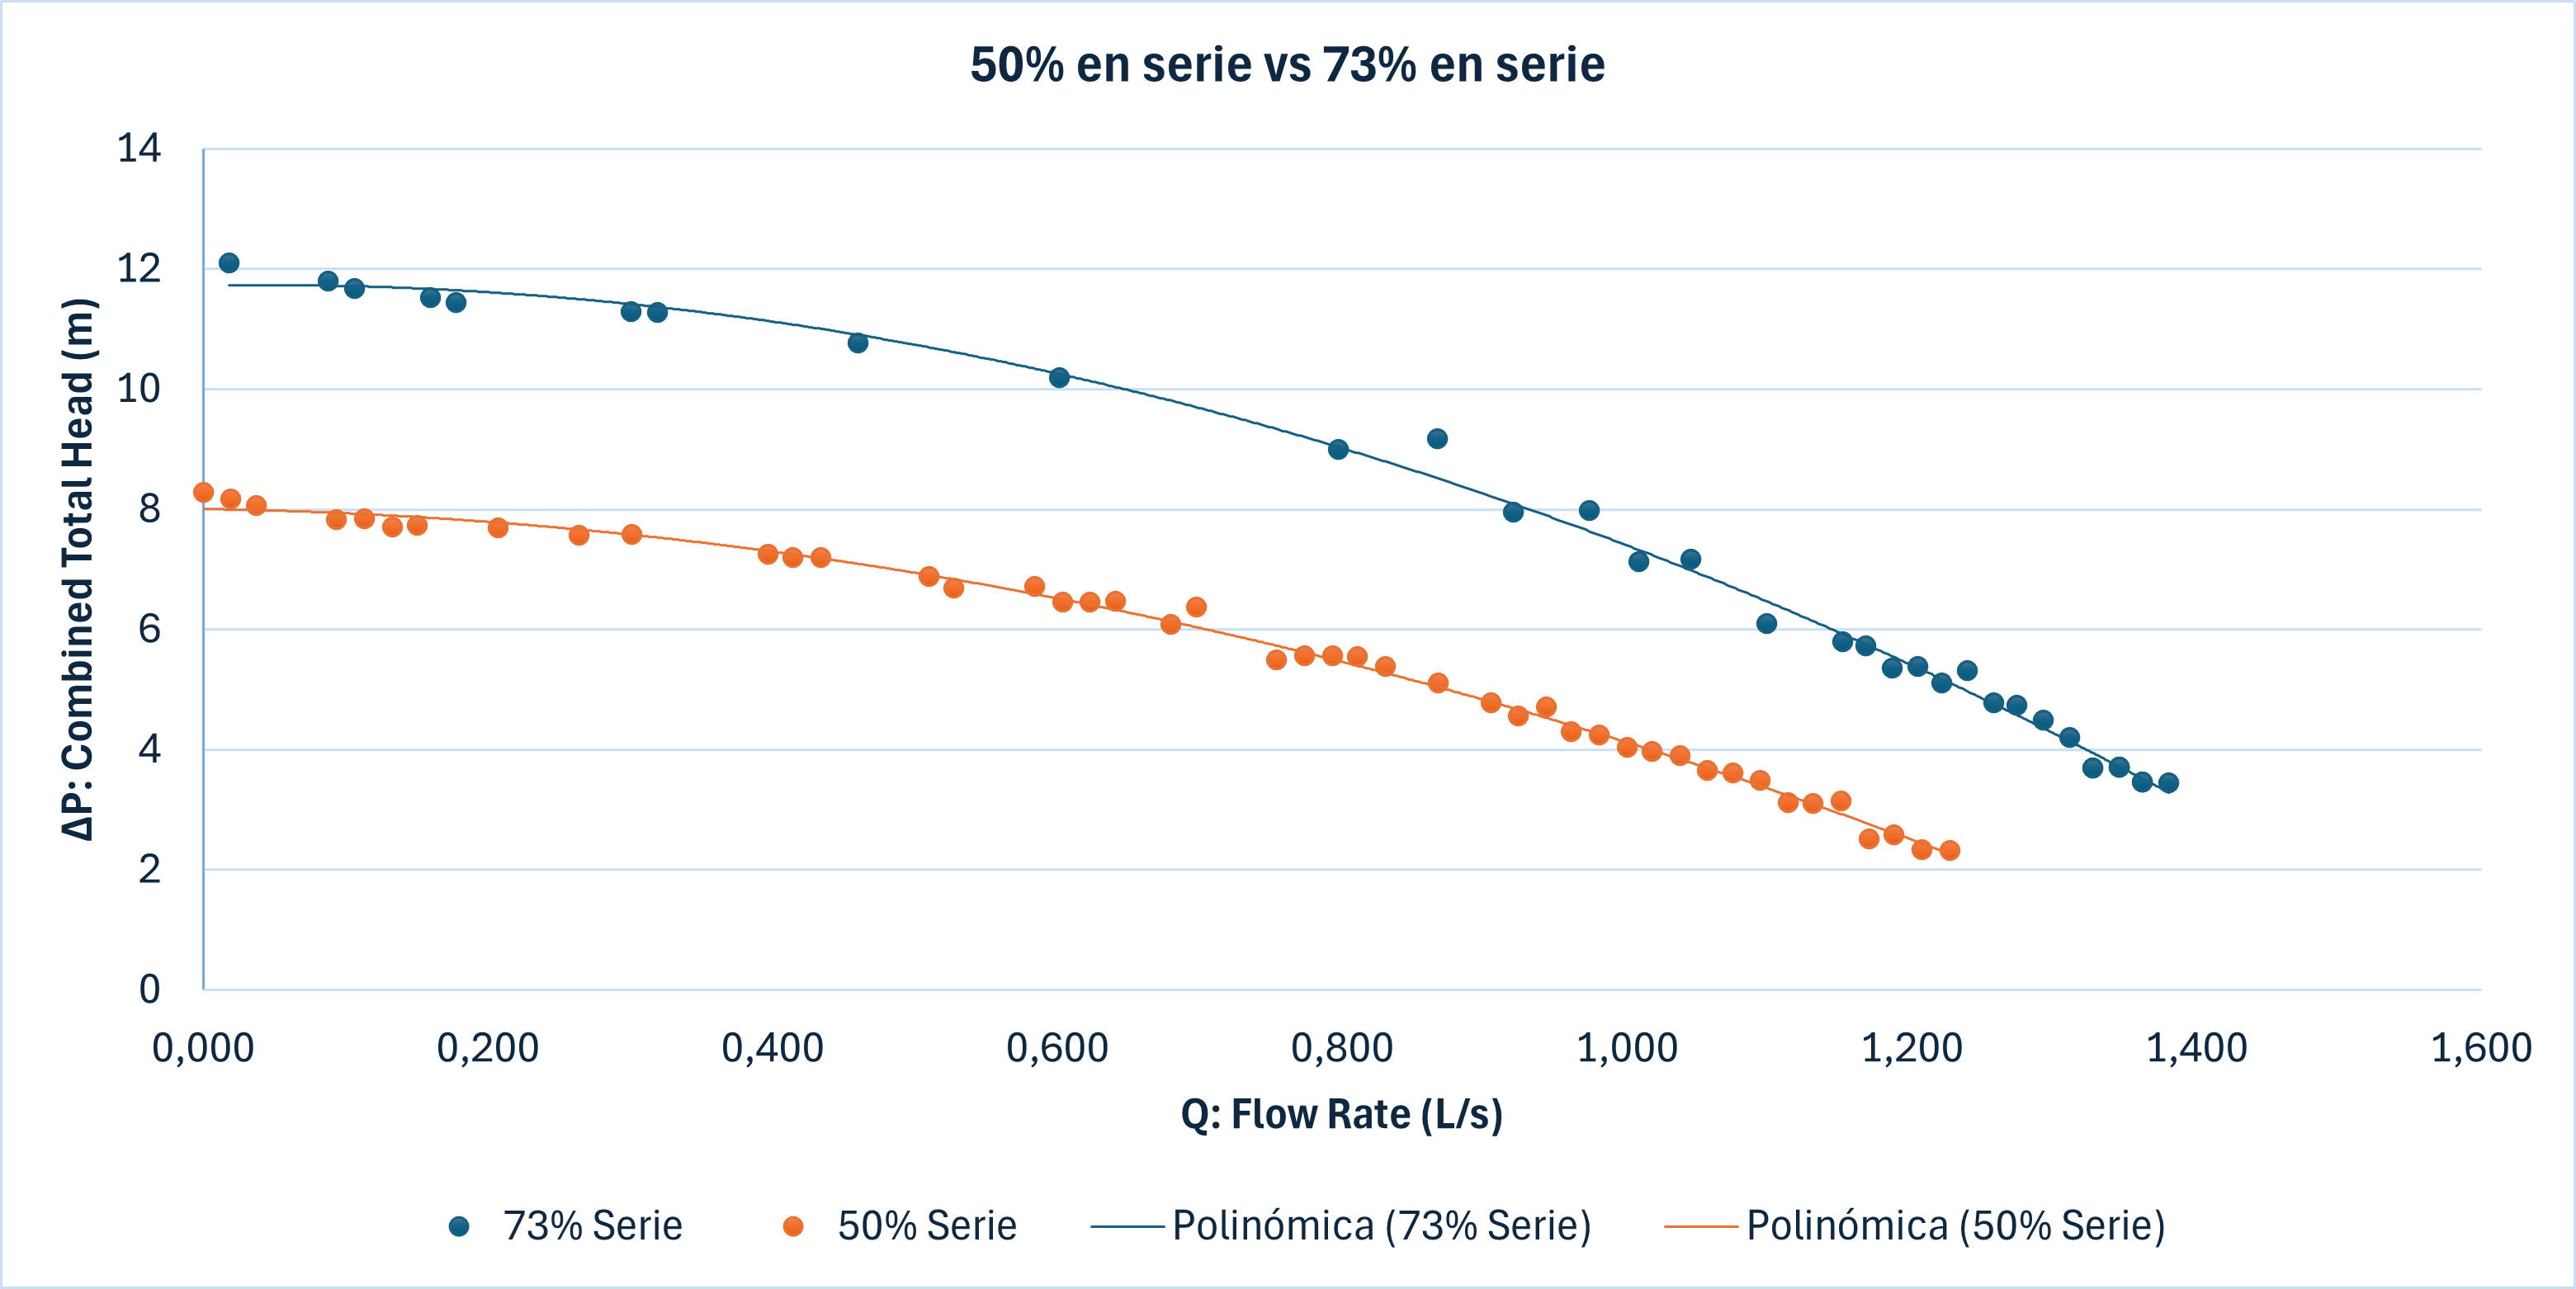
\includegraphics[width= 0.75 \textwidth]{Imagenes/BombasSerie Figura 2.png}
  \caption{Comparación de curvas características dimensionales de dos bombas en serie operando al $50\%$ y al $73\%$ de su caudal máximo.} 
  \label{fig: BombasSerie Figura 2}
\end{figure*}

En este apartado se contrastan los resultados de la configuración en serie operando al $50\%$ de su velocidad de giro máxima con al $73\%$. En la Figura \ref{fig: BombasSerie Figura 2} se aprecia que la forma que adquieren ambas gráficas es la misma puesto que la disposición es igual. Sin embargo, una está desplazada en diagonal, hacia la derecha y hacia arriba. Aquella situación en la que la velocidad de giro es mayor, es capaz de para un mismo caudal obtener una altura más grande, o lo que es lo mismo, si se desea superar una determinada altura, se precisa de una velocidad de giro mayor para tratar un caudal superior.

En este caso, para la curva del $50\%$ de la velocidad de giro los datos se encuentran uniformemente, además de ser la cantidad de datos de esta superior a la curva del $73\%$.

\subsubsection{Conclusiones}

\begin{itemize}
    \item La distribución de dos bombas en serie permite conseguir alturas mucho mayores para un mismo caudal que si se dispone de una sola bomba.
    \item El aumento de la velocidad de giro las bombas supone una mayor altura dado un caudal o poder tratar un caudal superior proporcionando una altura determinada.
\end{itemize}

\subsection{Bombas en operación en paralelo}
Finalmente se analiza el comportamiento de los grupos de bombeo en configuración paralela, evaluando cómo varía la relación entre el caudal volumétrico ($Q$) y la altura total generada ($\Delta P$) en función de distintos regímenes de funcionamiento. En concreto, se estudia el desempeño de dos bombas centrífugas trabajando a velocidades reducidas ($50\%$ y $73\%$ de su velocidad máxima), tanto de forma individual como en conjunto. Esta práctica se enmarca en el estudio experimental de las máquinas hidráulicas, y permite verificar los principios teóricos sobre el comportamiento de bombas en paralelo, como que el caudal total del sistema es la suma de los caudales individuales, mientras que la altura manométrica se mantiene aproximadamente constante respecto a la de una bomba individual.

\subsubsection{Comparación: $73 \%$ individual vs $73 \%$ paralelo}

\begin{figure*}[ht!]
  \centering
  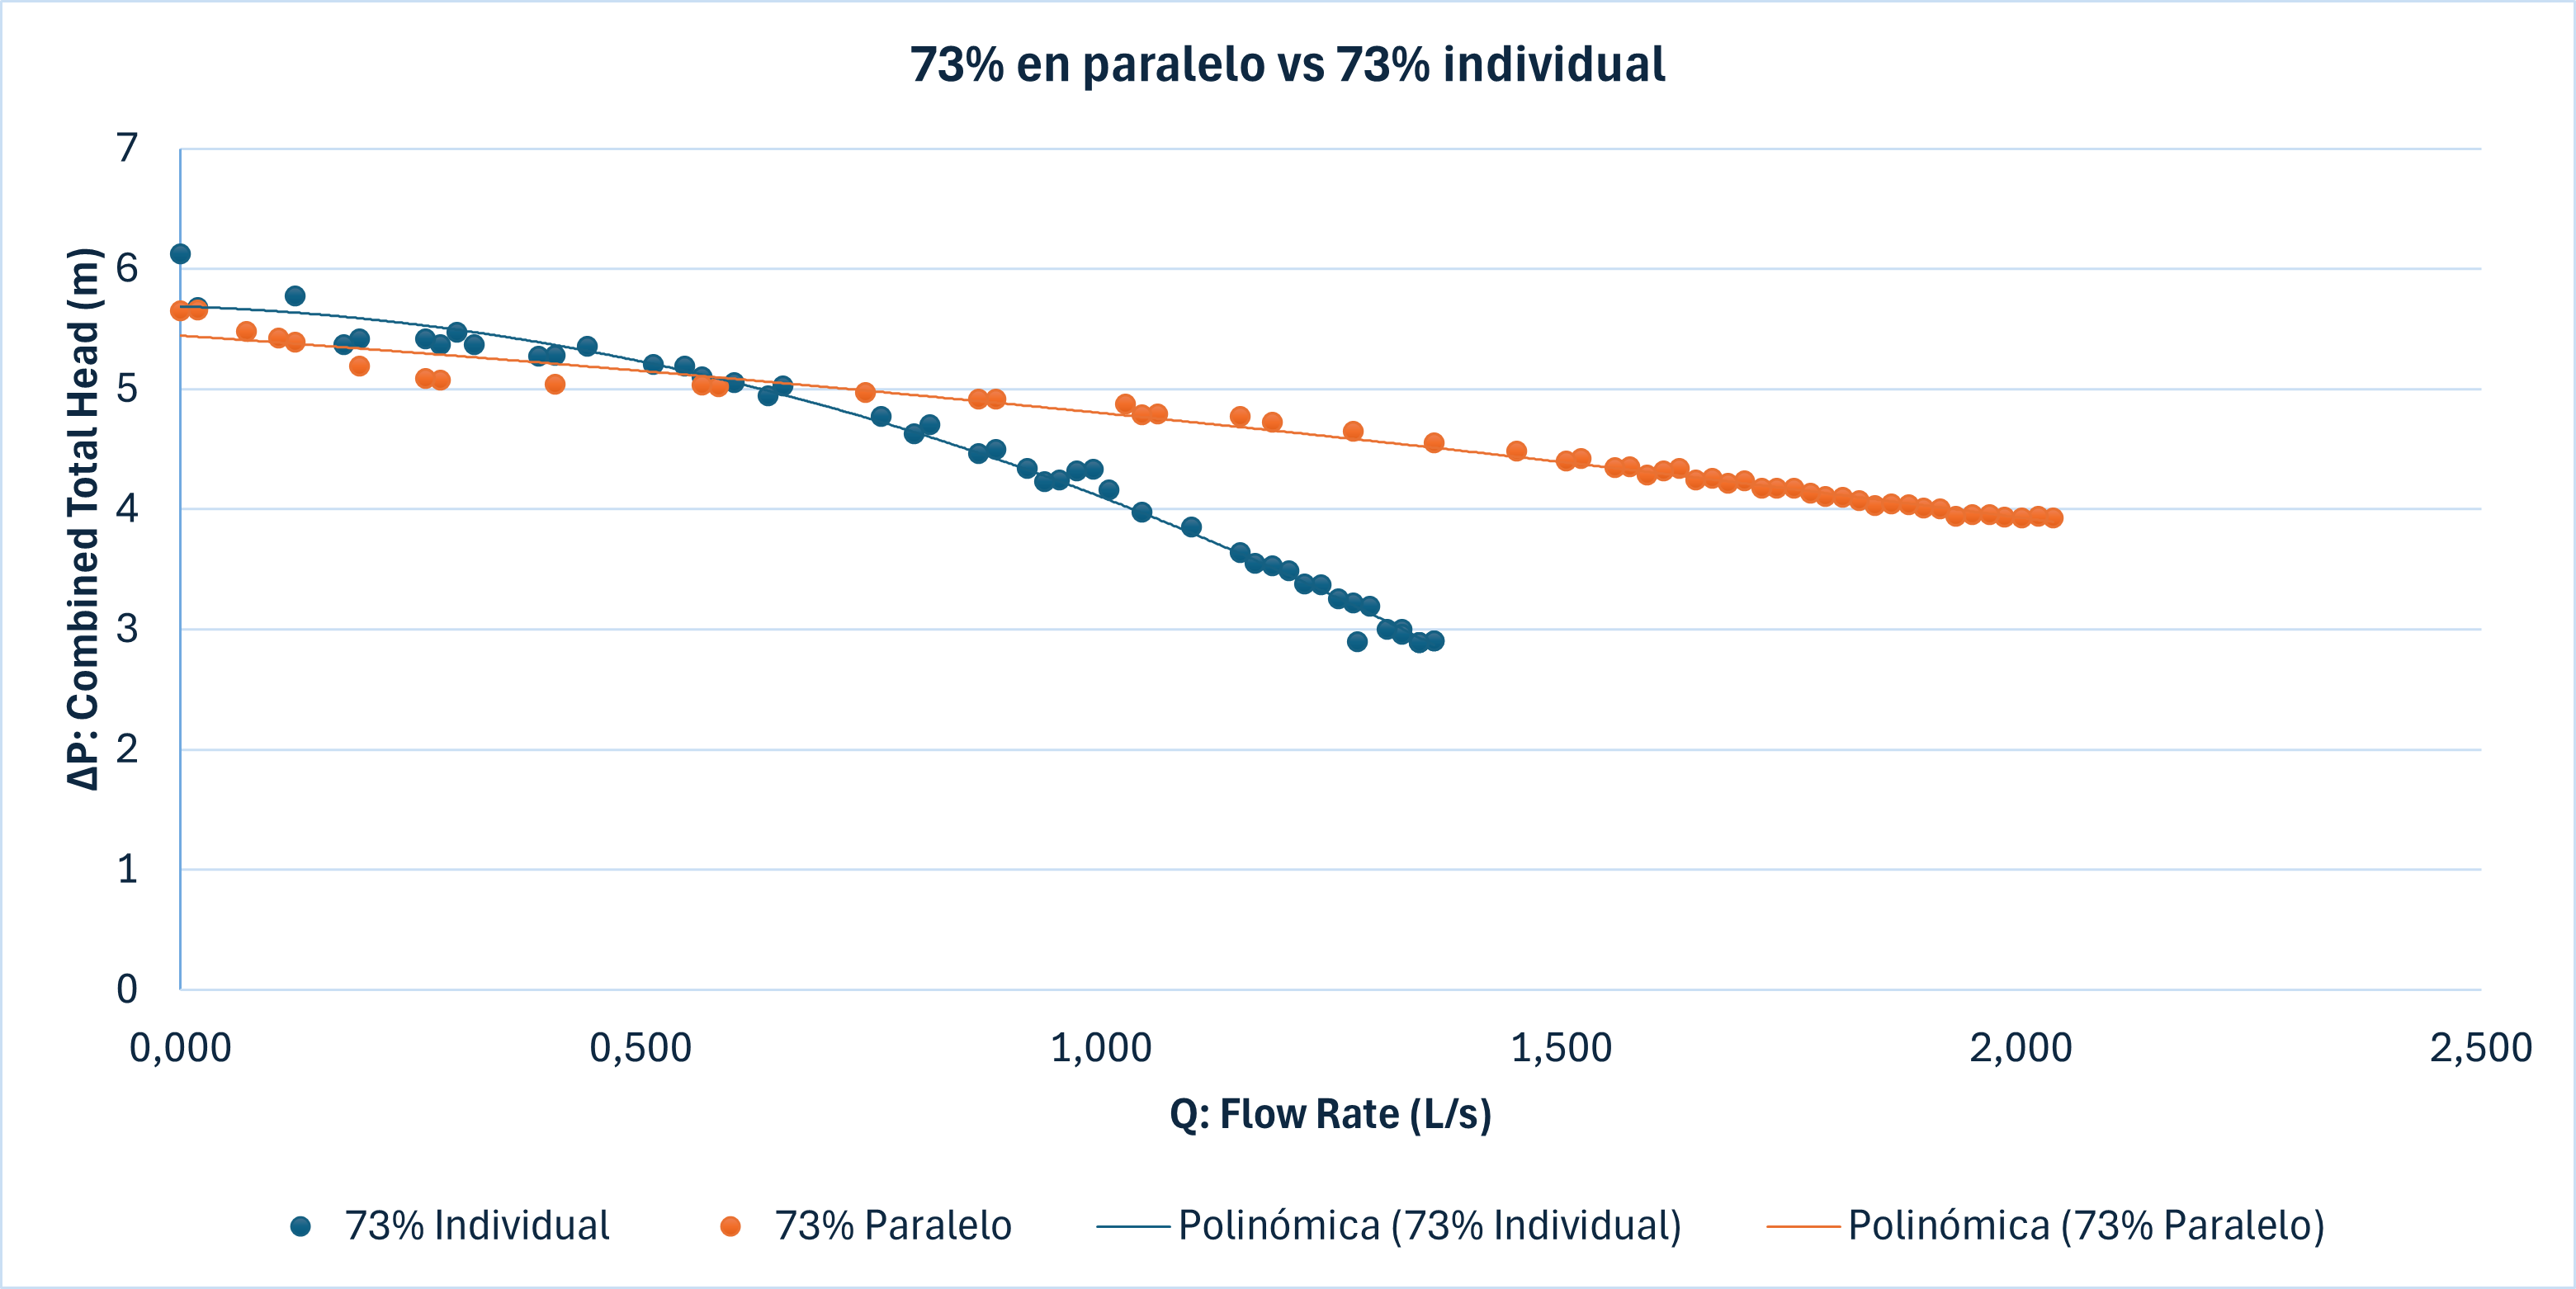
\includegraphics[width= 0.75 \textwidth]{Imagenes/BombasParalelo Figura 1.png}
  \caption{Comparación entre bomba individual y bombas en paralelo al 73\%}
  \label{fig: BombasParalelo Figura 1}
\end{figure*}

La figura \ref{fig: BombasParalelo Figura 1} muestra la comparación entre el funcionamiento de una bomba individual al $73\%$ de su velocidad máxima y dos bombas en paralelo a ese mismo régimen.

Se observa que:
\begin{itemize}
    \item •	A igualdad de presión ($\Delta P$), el sistema en paralelo proporciona un caudal significativamente mayor que una bomba individual.
    \item La curva correspondiente a la configuración paralela es más plana, indicando que el incremento de caudal no afecta en exceso la altura generada, hasta alcanzar un punto de caída más acusado.
    \item La forma polinómica de la curva del sistema en paralelo refleja una disminución más gradual de la altura con el aumento de caudal, debido a la capacidad compartida de trabajo entre las bombas.
\end{itemize}

Esto valida el principio teórico: las bombas en paralelo mantienen la misma presión que una bomba individual pero duplican el caudal (idealmente), aunque en la práctica surgen pequeñas desviaciones debidas a desequilibrios hidráulicos y pérdidas internas.

\subsubsection{Comparación: $50\%$ paralelo vs $73\%$ paralelo}

\begin{figure*}[ht!]
  \centering
  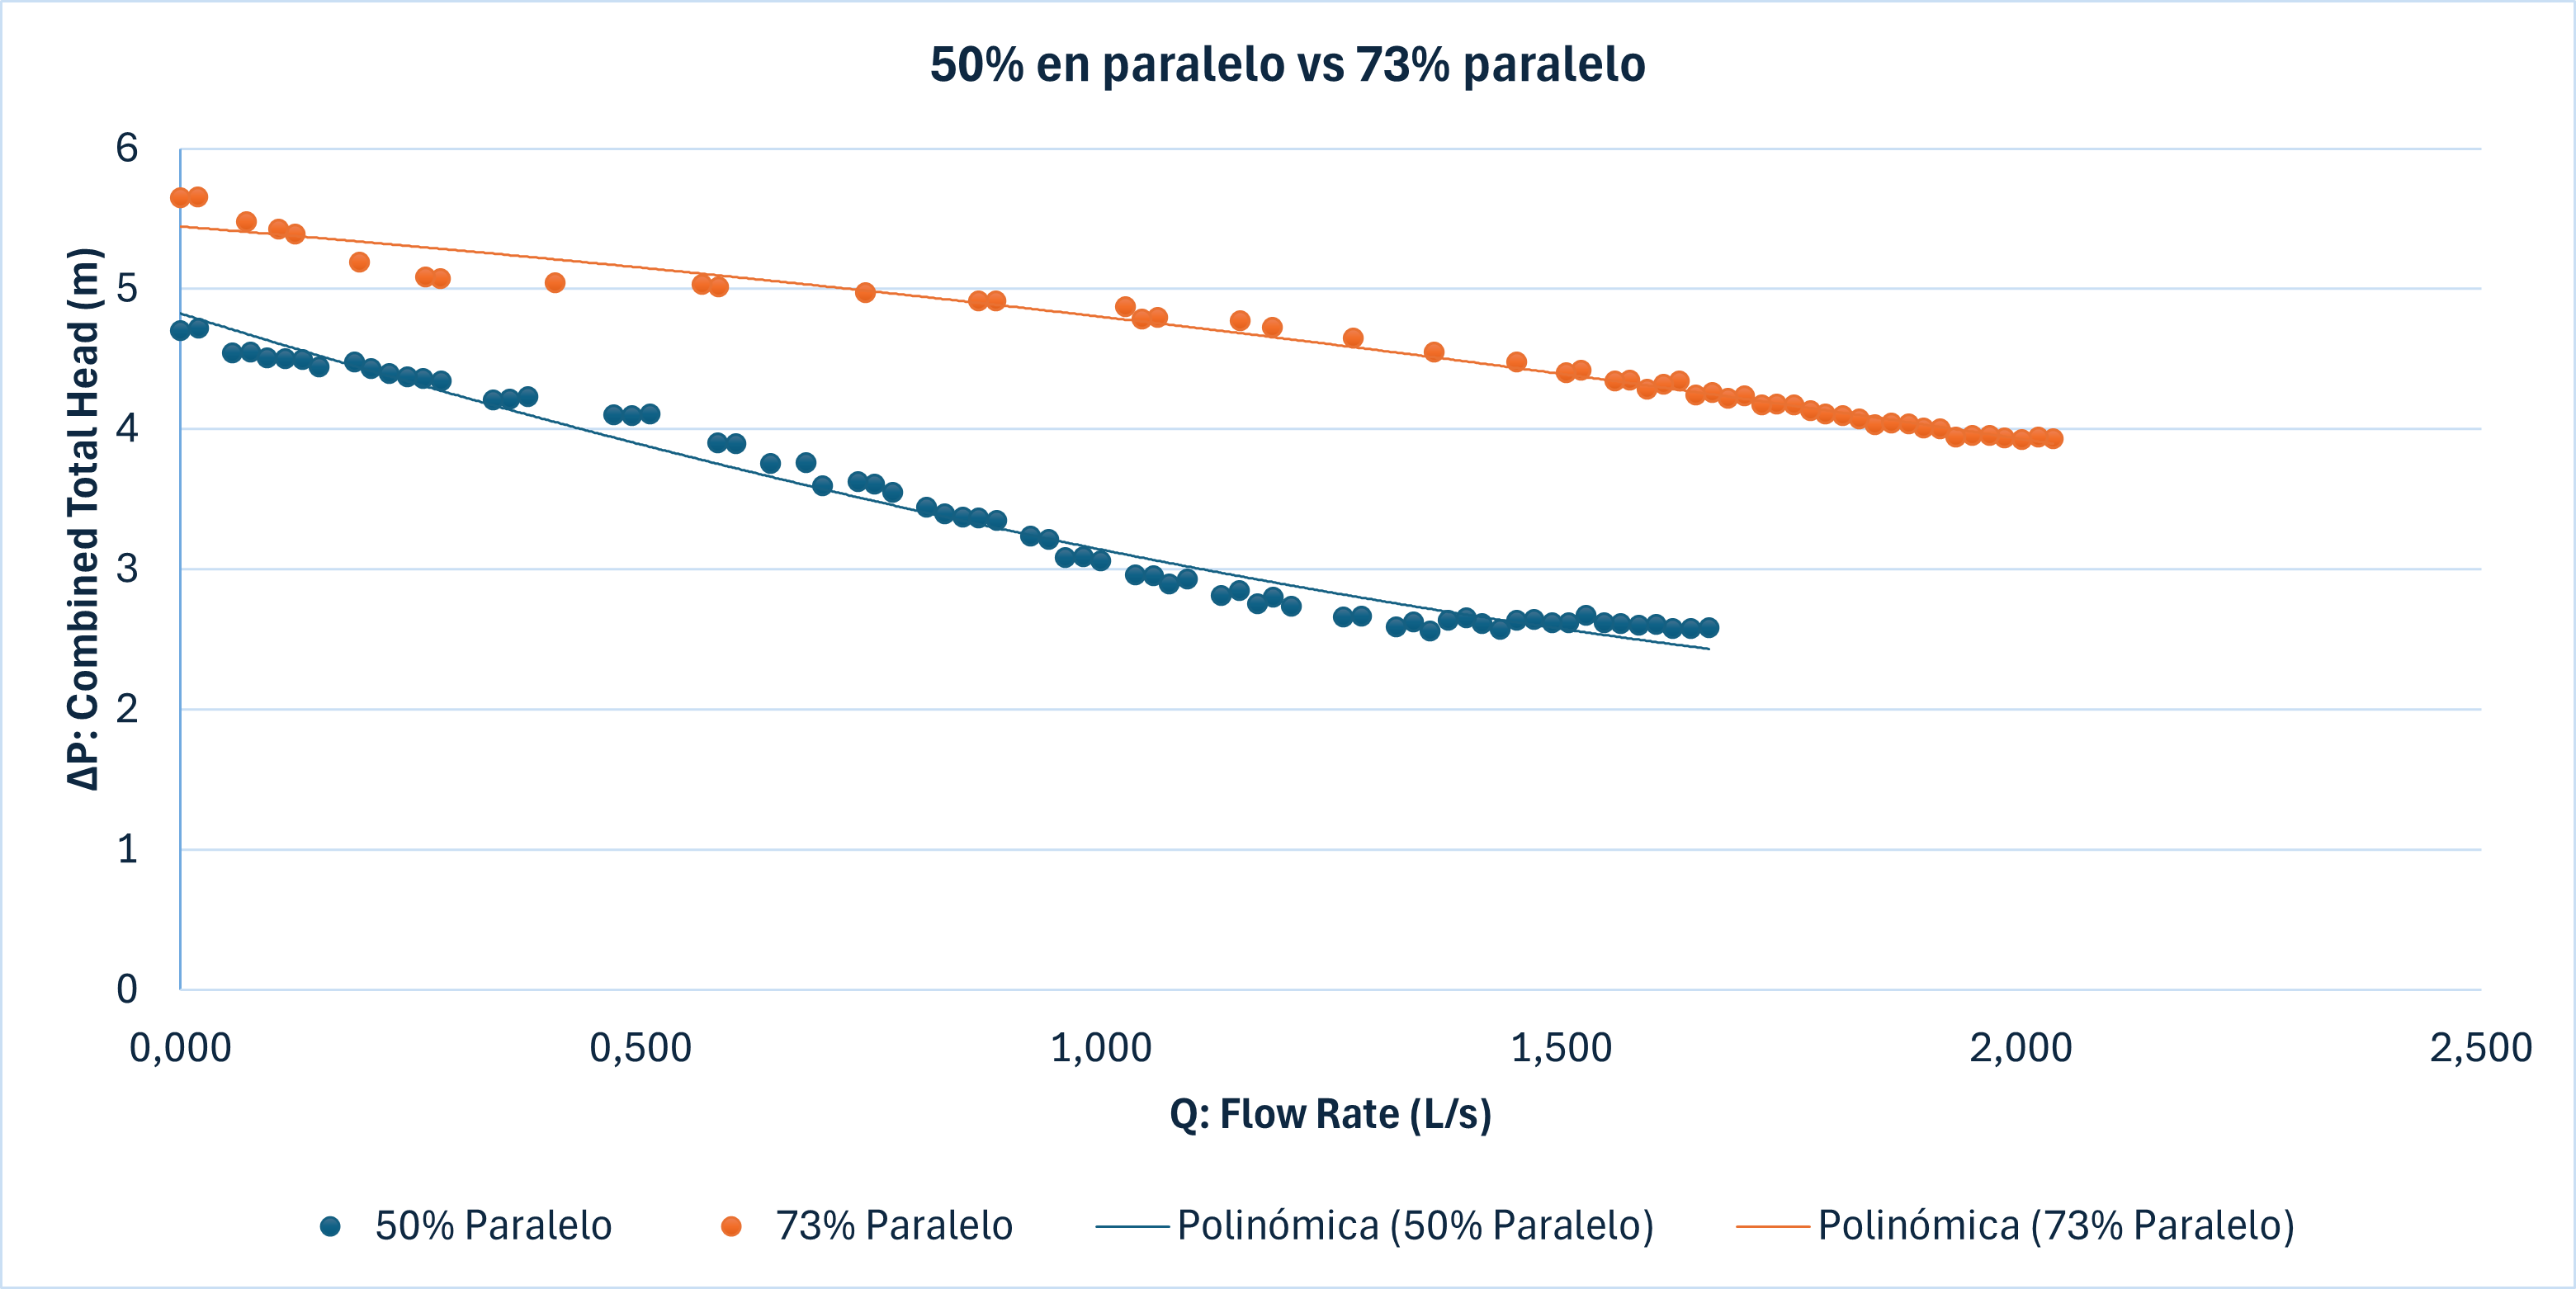
\includegraphics[width= 0.75 \textwidth]{Imagenes/BombasParalelo Figura 2.png}
  \caption{Comparación entre bombas en paralelo al 50\% y 73\% de velocidad máxima}
  \label{fig: BombasParalelo Figura 2}
\end{figure*}

La figura \ref{fig: BombasParalelo Figura 2} compara el comportamiento de dos bombas en paralelo, una funcionando al $50\%$ y otra al $73\%$ de la velocidad máxima.

Los resultados muestran:
\begin{itemize}
    \item A cualquier caudal dado, el sistema funcionando al $73\%$ ofrece mayores alturas manométricas, debido al mayor aporte energético del motor a esa velocidad.
    \item •	Ambas curvas siguen una tendencia decreciente, aunque la del $73\%$ se sitúa claramente por encima en todo el rango de caudales ensayado.
    \item La diferencia entre ambas curvas pone de manifiesto cómo el aumento de velocidad se traduce directamente en mayor rendimiento hidráulico, manteniéndose coherente con la teoría de semejanza para bombas centrífugas, donde la altura desarrollada varía con el cuadrado de la velocidad de giro.
\end{itemize}

Estos resultados demuestran que no solo la configuración hidráulica influye en el comportamiento del sistema, sino que la velocidad de funcionamiento tiene un impacto decisivo sobre la presión disponible y el rango útil de caudal.

\subsubsection{Conclusiones}
El estudio experimental confirma las hipótesis teóricas sobre el funcionamiento de bombas en paralelo. Al operar dos bombas a la vez:

\begin{itemize}
    \item Se duplica (o aumenta notablemente) el caudal, manteniendo una presión similar a la de una bomba individual.
    \item El rendimiento mejora notablemente respecto al funcionamiento aislado.
    \item La reducción de velocidad disminuye tanto la presión como el caudal, tal como predice la teoría de semejanza.
\end{itemize}

Este tipo de configuración es especialmente útil en sistemas que demandan flexibilidad de caudal sin alterar la presión del sistema, como redes de distribución o sistemas redundantes en procesos industriales. Los datos obtenidos, aunque con ligeras desviaciones respecto al comportamiento ideal, respaldan de forma general el marco teórico analizado en clase y constituyen una validación práctica valiosa de los principios hidráulicos fundamentales.

\onecolumn
\newpage
\twocolumn
{\LARGE Turbinas Hidráulicas \par}
\setcounter{section}{0}
\setcounter{subsection}{0}
\setcounter{subsubsection}{0}

En esta sección se recoge toda la información pertinente a la práctica sobre las turbinas hidráulicas.

\section{Introducción}
En este apartado se realiza una breve introducción, se mencionan los principales objetivos de la práctica y se desarrolla el fundamento teórico en el cual se basa.

Se ha estudiado el funcionamiento de una microturbina Pelton, un tipo de turbina hidráulica de acción utilizada para aprovechar saltos de agua elevados. El propósito principal de la práctica ha sido familiarizarse con el comportamiento y las características de este equipo, analizando variables como el caudal ($Q$), el par de frenado aplicado ($T$), la velocidad de rotación ($n$), la potencia desarrollada por la turbina ($W_t$) y el rendimiento ($\eta$). A través de la experimentación, se ha podido observar cómo la energía cinética del chorro de agua se transfiere a las cazoletas del rodete, transformándose en energía mecánica.

Esta práctica permite comprender los principios básicos de conversión de energía en sistemas hidráulicos y valorar la eficiencia de la turbina bajo distintas condiciones de operación.

\subsection{Objetivos}
Los principales objetivos de esta práctica se plantean a continuación:
\begin{itemize}
  \item Estudiar el funcionamiento y desempeño de una microturbina Pelton bajo diferentes condiciones de operación.
  \item Obtener y representar las curvas de potencia y rendimiento frente a velocidad angular del rodete, tanto en ejes dimensionales como adimensionales.
  \item Calcular el rendimiento máximo, y la velocidad específica de la turbina.
  \item Analizar y comentar los resultados obtenidos.
\end{itemize}

Es importante mencionar que, para llegar a cumplir todos los objetivos planteados, es necesario tener siempre presente la teoría vista en clase.

\subsection{Fundamento teórico}
Las turbinas hidráulicas se pueden dividir en dos tipos según su forma de transformar energía en el rodete: de acción y de reacción.

Las turbinas de acción únicamente intercambian energía cinética, mientras que las de reacción también pueden aprovechar la variación de presión del fluido.

La turbina Pelton pertenece al grupo de turbinas de acción, ya que no hay cambios de presión en el rodete. Toda la energía se transmite por el chorro de agua a alta velocidad que impacta en las cazoletas y genera el giro. Por ello, el diseño de los inyectores es clave. Este tipo de turbinas se utiliza para grandes saltos de agua y es la única capaz de operar en alturas extremas.

\section{Descripción del equipo de prácticas y metodología}
En esta sección se describe detalladamente el equipo utilizado en la práctica de turbinas hidráulicas. También se explica la metodología seguida para el correcto desarrollo de la práctica.

\subsection{Equipo de prácticas}

\begin{figure*}[ht!]
  \centering
  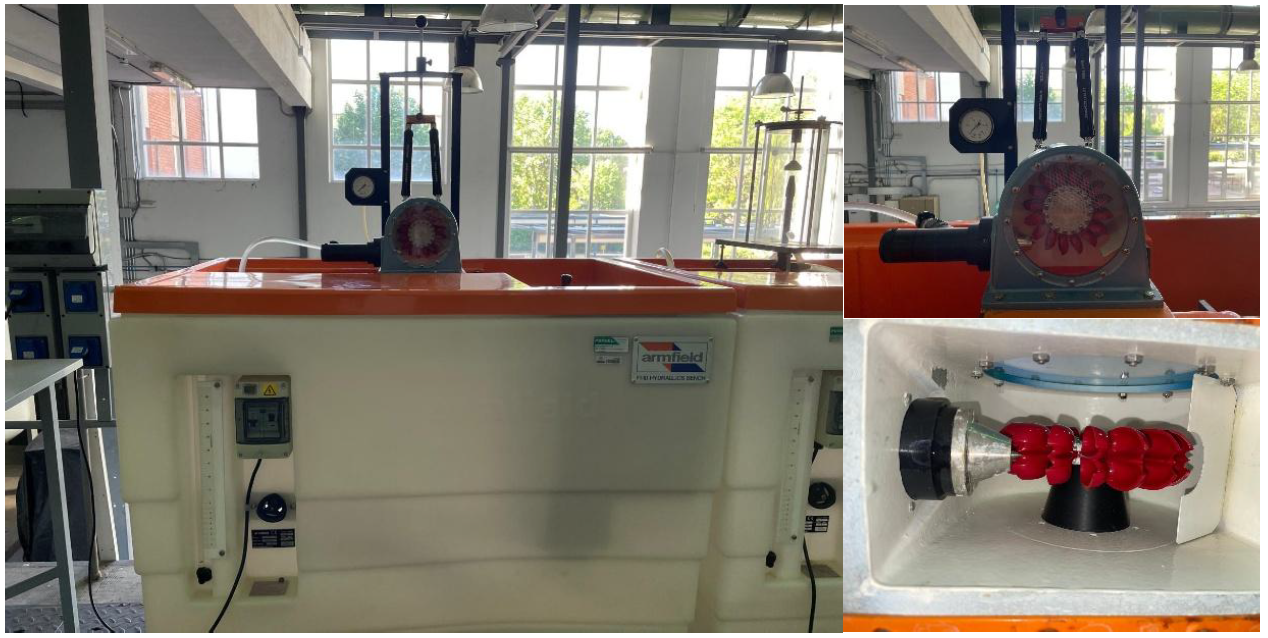
\includegraphics[width= 0.75 \textwidth]{Imagenes/Equipo de prácticas de turbina hidráulica.png}
  \caption{Equipo de practicas de turbina hidráulica} 
  \label{fig: Equipo de practicas de turbina hidráulica}
\end{figure*}

El equipo utilizado en esta práctica está diseñado para el análisis experimental de una microturbina tipo Pelton. El banco de ensayos se muestra en la Fig. \ref{fig: Equipo de practicas de turbina hidráulica} , y cuenta con todos los componentes necesarios para simular el funcionamiento real de una turbina de forma controlada en el laboratorio.

La instalación está compuesta por un circuito cerrado de agua, que incluye:
\begin{itemize}
  \item Un depósito principal de alimentación.
  \item Una bomba centrífuga que impulsa el agua hacia el inyector.
  \item Un inyector regulable mediante una válvula de aguja que genera un chorro de agua a alta presión.
  \item Un sistema de válvulas que permite ajustar y controlar el caudal.
  \item Un rodete tipo Pelton de $0,123\ m$ de diámetro ($D$), equipado con 16 cazoletas, sobre el que incide el chorro.
\end{itemize}

El rodete está alojado en una carcasa acrílica transparente, lo que permite observar visualmente el impacto del chorro sobre las cazoletas durante el ensayo. El eje del rodete está conectado a una polea de $0,05\ m$ de diámetro ($D_p$), sobre la cual actúa un sistema de freno mecánico por cinta, que se tensa entre dos dinamómetros. Este sistema permite aplicar un par resistente controlado, modificando así el régimen de giro de la turbina.

Para la medición de la velocidad de giro ($n$), se utiliza un tacómetro láser, que apunta a una marca reflectante adherida a la polea. Esta técnica no invasiva ofrece lecturas precisas del régimen de giro en revoluciones por minuto ($rpm$).

El par transmitido ($T$) se obtiene a partir de la fuerza de frenado ($F$). Por otro lado, el caudal se determina mediante el método volumétrico: se acumula una cantidad conocida de agua (en torno a 20 litros) en un depósito auxiliar, se cronometra el tiempo de llenado y se calcula el caudal como cociente entre volumen y tiempo. La lectura del volumen se realiza mediante una columna de agua graduada conectada al depósito.

Durante toda la práctica se mantuvo un salto neto ($H_n$) constante de aproximadamente 7 metros, condición fundamental para asegurar la comparabilidad de los datos tomados en los distintos ensayos.

Este equipo, de uso habitual en el laboratorio de máquinas hidráulicas de la ETSII-UPM, ofrece una plataforma robusta y precisa para el estudio del comportamiento de turbinas de acción bajo diferentes condiciones de carga.

\subsection{Metodología}
Uno de los objetivos principales de la práctica era obtener experimentalmente las curvas características de la turbina Pelton, específicamente las curvas de potencia y rendimiento en función de la velocidad de giro, bajo diferentes condiciones de caudal. Para ello, se realizaron mediciones siguiendo un procedimiento sistemático, manteniendo siempre una altura neta constante de aproximadamente 7 metros.

Durante el desarrollo de la práctica se trabajó con cinco valores distintos de caudal. Para cada uno de ellos se realizaron entre 5 y 6 mediciones variando el par de frenado, lo que ha permitido obtener diferentes puntos de operación sobre la curva correspondiente.

A continuación, se detalla el procedimiento seguido en cada uno de los ensayos:
\begin{enumerate}
  \item Fijación del caudal: Se ajustó la válvula del depósito de alimentación hasta alcanzar el caudal deseado. El valor del caudal se determinó como se ha mencionado anteriormente. La lectura del volumen se realizó mediante una columna de agua graduada, y el cronometraje se hizo mediante la función de cronómetro de un teléfono móvil.
  \item Ajuste de la válvula de aguja: Con el caudal fijado, se abre o cierra la válvula de aguja para obtener el salto neto fijado previamente.
  \item Ajuste de la fuerza de frenado: Con el caudal y el salto neto fijados, se modificó el par de frenado aplicando distintas tensiones sobre la cinta de freno que rodea la polea del eje. Este par se controlaba mediante el ajuste vertical de los dinamómetros, introduciendo diferentes resistencias al giro.
  \item Medición de la velocidad de giro: Para cada nivel de freno, se midió el régimen de giro del eje utilizando un tacómetro láser, apuntando a una marca reflectante en la polea.
  \item Medición de la fuerza de frenado: Para obtener la fuerza de frenado era necesario restar el valor que marcaba el dinamómetro de la izquierda menos el valor que marcaba el de la derecha. Sin embargo, la resta de ambos no era la fuerza real de frenado, ya que se debía tener en cuenta una falta de precisión en el dinamómetro de la derecha de $0.25\ N$. Por lo tanto, la fuerza real de frenado se calculaba siguiendo la siguiente fórmula:
  \begin{equation}
    F = (F_1 - F_2) - 0.25
  \end{equation}
  \item Registro y repetición: Este procedimiento se repitió para cada uno de los cinco caudales, asegurando que en todos los casos el salto neto permaneciese constante. Para cada valor de caudal se generaron así varias combinaciones de par y velocidad, obteniéndose suficientes datos como para construir las curvas características.
\end{enumerate}

\begin{table*}[ht!]
  \centering
  \caption{Medidas tomadas y valores relevantes para la representación de las curvas}
  \label{tab: Medidas tomadas y valores relevantes para la representación de las curvas}
  \begin{tabular}{|c|c|c|c|c|c|c|c|c|c|c|c|c|}
    \hline
    $V$ [L] & $t$ [s] & $Q$ [L/s] & $n$ [rpm] & $\omega$ [rad/s] & $F$ [N] & $T$ [Nm] & $W_t$ [W] & $W_h$ [W] & $\eta$ & $C_P$ & $C_v$ & $\omega_s$ \\
    \hline
    \multirow{6}{*}{15} & \multirow{6}{*}{81} & \multirow{6}{*}{0.185} & 1425 & 149.2 & 0.00 & 0.000 & 0.000 & 12.691 & 0.00 & 0.0000 & 2.2150 & 0.000 \\
    \cline{4-13}
    & & & 1335 & 139.8 & 0.50 & 0.025 & 3.495 & 12.691 & 0.28 & 0.0004 & 2.0751 & 0.042 \\
    \cline{4-13}
    & & & 1130 & 118.3 & 1.25 & 0.063 & 7.396 & 12.691 & 0.58 & 0.0009 & 1.7564 & 0.052 \\
    \cline{4-13}
    & & & 972  & 101.8 & 1.80 & 0.090 & 9.161 & 12.691 & 0.72 & 0.0011 & 1.5108 & 0.049 \\
    \cline{4-13}
    & & & 393  & 41.2  & 2.50 & 0.125 & 5.144 & 12.691 & 0.41 & 0.0006 & 0.6109 & 0.015 \\
    \cline{4-13}
    & & & 138  & 14.5  & 3.25 & 0.163 & 2.348 & 12.691 & 0.19 & 0.0003 & 0.2145 & 0.004 \\
    \hline
    \multirow{7}{*}{20} & \multirow{7}{*}{68.7} & \multirow{7}{*}{0.291} & 1610 & 168.6 & 0.00 & 0.000 & 0.000 & 19.951 & 0.00 & 0.0000 & 2.5025 & 0.000 \\
    \cline{4-13}
    & & & 1520 & 159.2 & 0.85 & 0.043 & 6.765 & 19.951 & 0.34 & 0.0008 & 2.3626 & 0.066 \\
    \cline{4-13}
    & & & 1160 & 121.5 & 2.76 & 0.138 & 16.764 & 19.951 & 0.84 & 0.0020 & 1.8031 & 0.080 \\
    \cline{4-13}
    & & & 830  & 86.9  & 4.00 & 0.200 & 17.383 & 19.951 & 0.87 & 0.0020 & 1.2901 & 0.058 \\
    \cline{4-13}
    & & & 497  & 52.0  & 5.00 & 0.250 & 13.011 & 19.951 & 0.65 & 0.0015 & 0.7725 & 0.030 \\
    \cline{4-13}
    & & & 100  & 10.5  & 5.75 & 0.288 & 3.011 & 19.951 & 0.15 & 0.0004 & 0.1554 & 0.003 \\
    \cline{4-13}
    & & & 0    & 0.0   & 6.25 & 0.313 & 0.000 & 19.951 & 0.00 & 0.0000 & 0.0000 & 0.000 \\
    \hline
    \multirow{6}{*}{20} & \multirow{6}{*}{45.64} & \multirow{6}{*}{0.438} & 1645 & 172.3 & 0.00 & 0.000 & 0.000 & 30.032 & 0.00 & 0.0000 & 2.5569 & 0.000 \\
    \cline{4-13}
    & & & 1530 & 160.2 & 1.35 & 0.068 & 10.815 & 30.032 & 0.36 & 0.0013 & 2.3782 & 0.084 \\
    \cline{4-13}
    & & & 1400 & 146.6 & 2.55 & 0.128 & 18.692 & 30.032 & 0.62 & 0.0022 & 2.1761 & 0.101 \\
    \cline{4-13}
    & & & 1220 & 127.8 & 3.75 & 0.188 & 23.955 & 30.032 & 0.80 & 0.0028 & 1.8963 & 0.100 \\
    \cline{4-13}
    & & & 1035 & 108.4 & 4.95 & 0.248 & 26.825 & 30.032 & 0.89 & 0.0031 & 1.6088 & 0.090 \\
    \cline{4-13}
    & & & 770  & 80.6  & 6.15 & 0.308 & 24.795 & 30.032 & 0.83 & 0.0029 & 1.1969 & 0.064 \\
    \hline
    \multirow{6}{*}{15} & \multirow{6}{*}{29.05} & \multirow{6}{*}{0.516} & 1667 & 174.6 & 0.00 & 0.000 & 0.000 & 35.387 & 0.00 & 0.0000 & 2.5911 & 0.000 \\
    \cline{4-13}
    & & & 1552 & 162.5 & 1.25 & 0.063 & 10.158 & 35.387 & 0.29 & 0.0012 & 2.4124 & 0.083 \\
    \cline{4-13}
    & & & 1486 & 155.6 & 2.00 & 0.100 & 15.561 & 35.387 & 0.44 & 0.0018 & 2.3098 & 0.098 \\
    \cline{4-13}
    & & & 1383 & 144.8 & 3.50 & 0.175 & 25.345 & 35.387 & 0.72 & 0.0029 & 2.1497 & 0.117 \\
    \cline{4-13}
    & & & 799  & 83.7  & 7.75 & 0.388 & 32.423 & 35.387 & 0.92 & 0.0038 & 1.2419 & 0.076 \\
    \cline{4-13}
    & & & 0    & 0.0   & 10.0 & 0.500 & 0.000  & 35.387 & 0.00 & 0.0000 & 0.0000 & 0.000 \\
    \hline
    \multirow{6}{*}{20} & \multirow{6}{*}{34.98} & \multirow{6}{*}{0.572} & 1690 & 177.0 & 0.00 & 0.000 & 0.000 & 39.184 & 0.00 & 0.0000 & 2.6269 & 0.000 \\
    \cline{4-13}
    & & & 1585 & 166.0 & 1.35 & 0.068 & 11.204 & 39.184 & 0.29 & 0.0013 & 2.4637 & 0.089 \\
    \cline{4-13}
    & & & 1490 & 156.0 & 2.55 & 0.128 & 19.894 & 39.184 & 0.51 & 0.0023 & 2.3160 & 0.111 \\
    \cline{4-13}
    & & & 1400 & 146.6 & 3.75 & 0.188 & 27.489 & 39.184 & 0.70 & 0.0032 & 2.1761 & 0.123 \\
    \cline{4-13}
    & & & 1285 & 134.6 & 4.95 & 0.248 & 33.305 & 39.184 & 0.85 & 0.0039 & 1.9973 & 0.124 \\
    \cline{4-13}
    & & & 1140 & 119.4 & 5.95 & 0.298 & 35.516 & 39.184 & 0.91 & 0.0041 & 1.7720 & 0.114 \\
    \hline
  \end{tabular}
\end{table*}


\section{Resultados}
En esta sección se describen los procedimientos seguidos para la obtención y representación de las curvas características de la microturbina, en particular las curvas de potencia y rendimiento en función de la velocidad angular, para distintos valores de caudal.

Se llevaron a cabo ensayos con cinco valores distintos de caudal. Para cada uno de ellos, se obtuvieron varios puntos experimentales mediante la variación del par de frenado aplicado, lo que permitió generar un conjunto de datos adecuado para trazar las curvas correspondientes.

\subsection{Obtención del caudal}
En primer lugar, se mide el caudal ($Q$) utilizando el método volumétrico, es decir, cronometrando el tiempo necesario para llenar un volumen determinado:
\begin{equation}
  Q = \frac{V}{t}
\end{equation}
Es preciso mencionar que, para los dos caudales más grandes, no se tomaron datos con grandes valores de fuerza, lo que dificulta la representación de las curvas características de la turbina. Sin embargo, utilizando funciones cuadráticas, se obtienen buenos resultados.

\subsection{Cálculo del par aplicado}
El par resistente aplicado ($T$) se calcula como el producto entre la fuerza de frenado corregida ($F$) y el diámetro de la polea ($D_p$) sobre la que actúa el sistema de freno. Cabe mencionar que se utiliza la medida del diámetro y no la del radio debido a que se dispone de dos dinamómetros separados mediante el diámetro.
\begin{equation}
  T = F \cdot D_p
\end{equation}
El valor del par que se obtiene en $[Nm]$ se utilizará para calcular la potencia desarrollada por la turbina ($W_t$).

\subsection{Cálculo de la potencia}
Con el caudal fijado, se procede a medir la velocidad de giro del rodete ($n$) y la fuerza de frenado ($F$) aplicada a través del sistema mecánico con dinamómetros.

A partir de estos datos, se calcula la potencia desarrollada por la turbina ($W_t$) en vatios $[W]$ mediante el producto entre el par resistente ($T$) aplicado y la velocidad angular ($\omega$) en $[rad/s]$:
\begin{equation}
  W_t = T \cdot \omega
  \label{eq: Turbinas - Ecuacion 4}
\end{equation}
En la ecuación (\ref{eq: Turbinas - Ecuacion 4}), la velocidad angular $\omega$ se ha obtenido a partir de la velocidad de giro del rodete $n$ en $[rpm]$ medida con el tacómetro:
\begin{equation}
  \omega = \frac{2 \pi}{60} n
\end{equation}

\subsection{Cálculo del rendimiento}
Una vez calculada la potencia desarrollada por la turbina, se obtiene el rendimiento de la turbina como la relación entre dicha potencia ($W_t$) y la potencia intercambiada por el rodete ($W_h$).
\begin{equation}
  \eta = \frac{W_t}{W_h}
  \label{eq: Turbinas - Ecuacion 6}
\end{equation}

La potencia intercambiada por el rodete ($W_h$) se expresa de la siguiente forma:
\begin{equation}
  W_h = \rho g Q H_n
\end{equation}
Donde:
\begin{itemize}
  \item $\rho$ es la densidad del agua $[kg/m^3]$
  \item $g$ es la aceleración de la gravedad $[m/s^2]$
  \item $Q$ es el caudal $[m^3/s]$
  \item $H_n$ es el salto neto constante mantenido durante toda la práctica $[m]$
\end{itemize}

\subsection{Cálculo de los parámetros adimensionales}
Por último, se han calculado los parámetros adimensionales necesarios para representar todas las curvas de interés. Estos son el coeficiente de potencia ($C_p$) y el coeficiente de velocidad ($C_v$), y se obtienen a partir de las siguientes expresiones:
\begin{equation}
  C_p = \frac{W_t \sqrt{\rho}}{\Delta p^{\frac{3}{2}}D^2}
  \label{eq: Turbinas - Ecuacion 8}
\end{equation}
\begin{equation}
  C_v = \frac{\omega D \sqrt{\rho}}{\sqrt{\Delta p}}
  \label{eq: Turbinas - Ecuacion 9}
\end{equation}

Donde $D$ representa el diámetro del rodete y $\Delta p$ representa el salto de presiones en $[Pa]$ calculado de la siguiente forma:
\begin{equation}
  \Delta p = \rho g H_n
\end{equation}

Finalmente, los resultados obtenidos se representan gráficamente, generando para cada valor de caudal una curva de potencia frente a velocidad angular y una curva de rendimiento frente a velocidad angular tanto en ejes dimensionales como adimensionales.

\subsection{Curvas obtenidas}
En el caso dimensional, se han representado las siguientes curvas:
\begin{itemize}
  \item Potencia desarrollada por la turbina ($W_t$) frente a la velocidad de giro $n$.
  \item Rendimiento $\eta$ frente a la velocidad de giro $n$.
\end{itemize}

Mientras que, en el caso adimensional, se han trazado las siguientes curvas:
\begin{itemize}
  \item Coeficiente de potencia $C_p$ frente al coeficiente de velocidad $C_v$.
  \item Rendimiento $\eta$ frente al coeficiente de velocidad $C_v$.
\end{itemize}

\begin{figure*}[ht!]
  \centering
  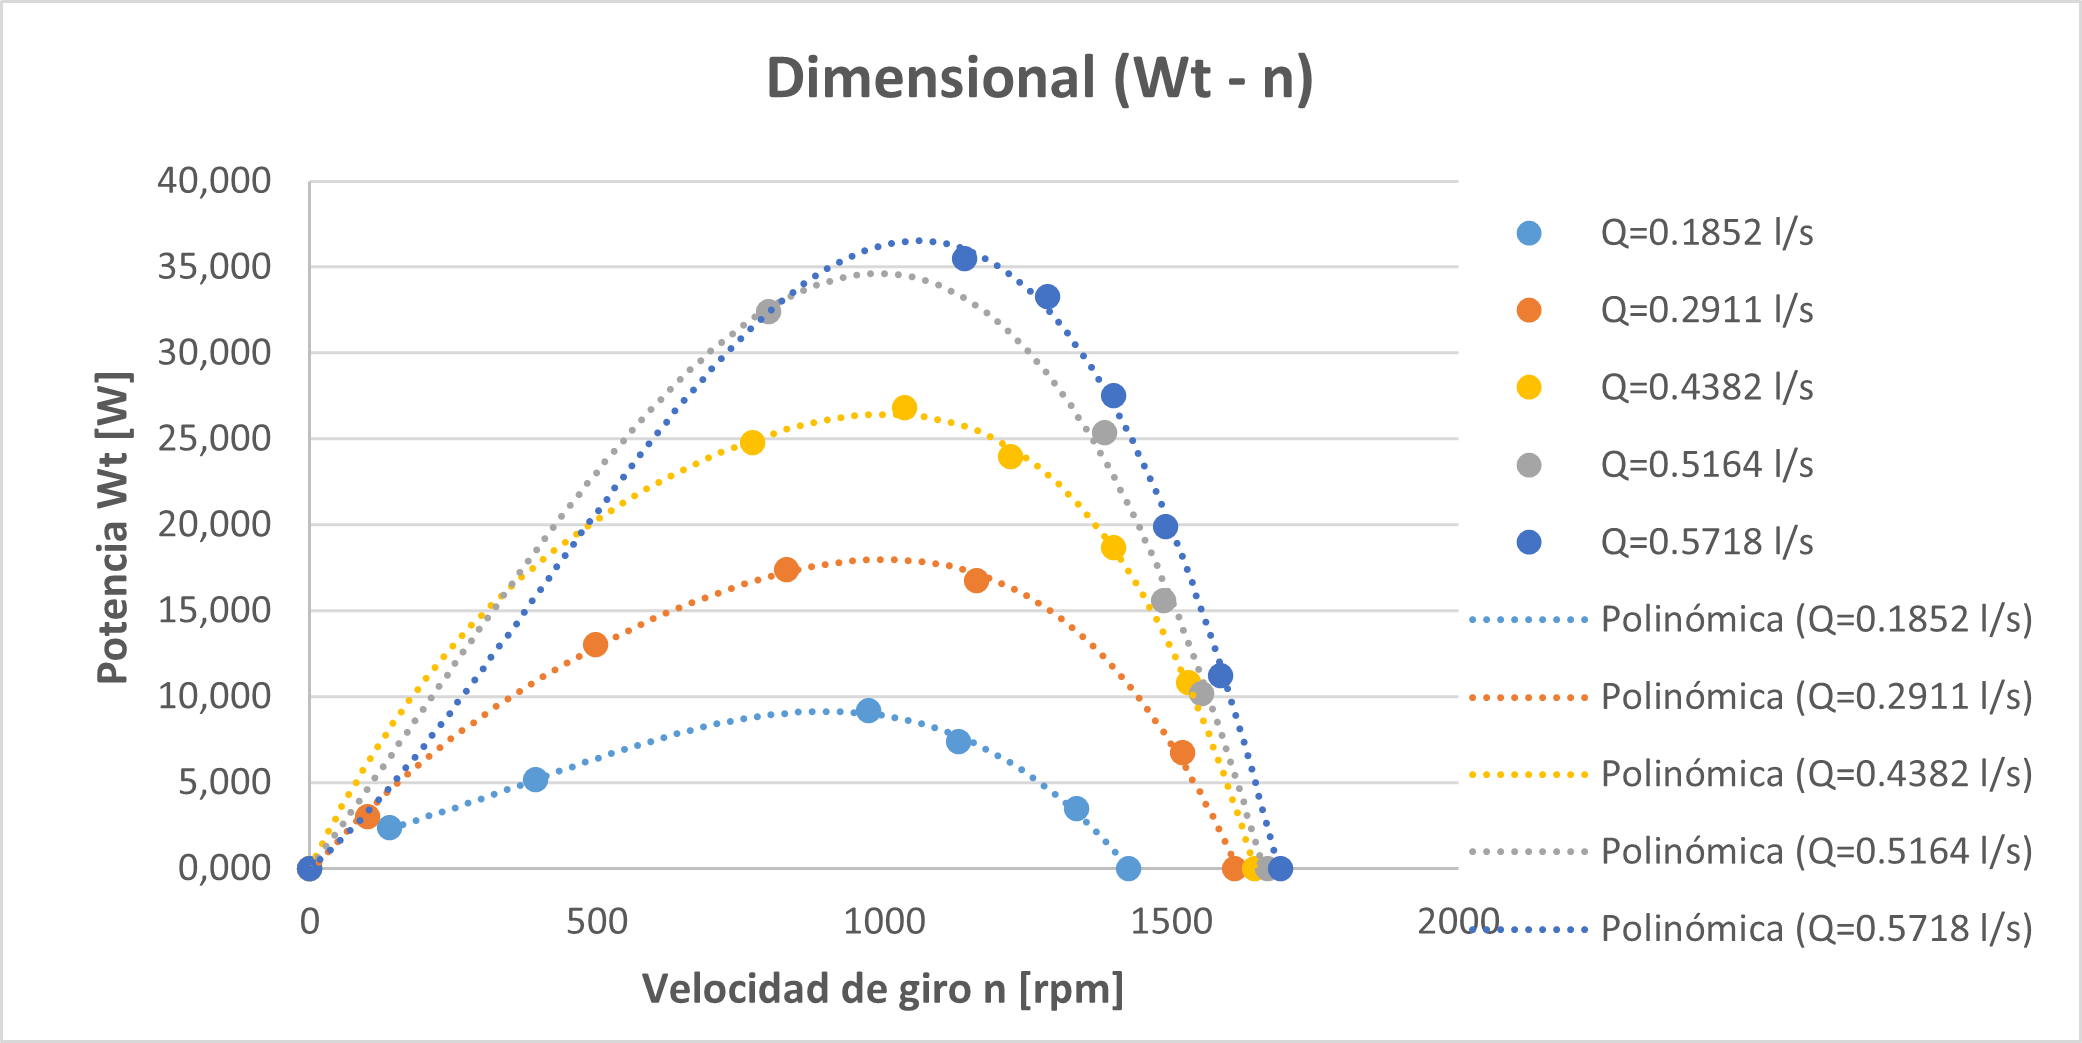
\includegraphics[width= 0.75 \textwidth]{Imagenes/Curvas de potencia frente a velocidad de giro.png}
  \caption{Curvas de potencia ($W_t$) frente a velocidad de giro ($n$)} 
  \label{fig: Curvas de potencia frente a velocidad de giro}
\end{figure*}

En primer lugar, se representa la potencia desarrollada por la turbina frente a la velocidad de giro para cada uno de los caudales medidos en la Fig. \ref{fig: Curvas de potencia frente a velocidad de giro}. Como cabía esperar, a mayor caudal, mayor potencia desarrollada por la turbina.

Por otra parte, se observa un comportamiento similar para cada una de las cinco curvas, lo que sugiere una correcta toma de datos por parte del equipo. Además, este comportamiento concuerda con lo visto en la parte teórica de la asignatura.

La curva de potencia frente a régimen de giro debe mostrar una función creciente a medida que aumenta la velocidad de giro hasta llegar a un máximo en torno a la mitad del valor máximo de régimen de giro de la turbina. Una vez alcanzado ese valor, la función decrece hasta llegar a 0 vatios desarrollados cuando no se aplica fuerza de frenado. En este punto, la velocidad de giro del rodete es la máxima alcanzable para el valor del caudal con el que se está trabajando.

También se puede observar que, a mayor caudal, mayor es la velocidad de giro óptima.

En cuanto a los rangos de potencia desarrollada por la turbina y velocidad de giro de la misma, se han obtenido potencias inferiores a los $40\ W$, llegando a un máximo de $35.5\ W$ para el mayor caudal a una velocidad de giro de $1140\ rpm$. Este rango de potencias es el esperado para una microturbina Pelton de estas características. El rango de velocidad de giro concuerda con lo especificado en el guion de prácticas, aunque no se haya llegado al régimen de giro máximo de $2000\ rpm$.

\begin{figure*}[ht!]
  \centering
  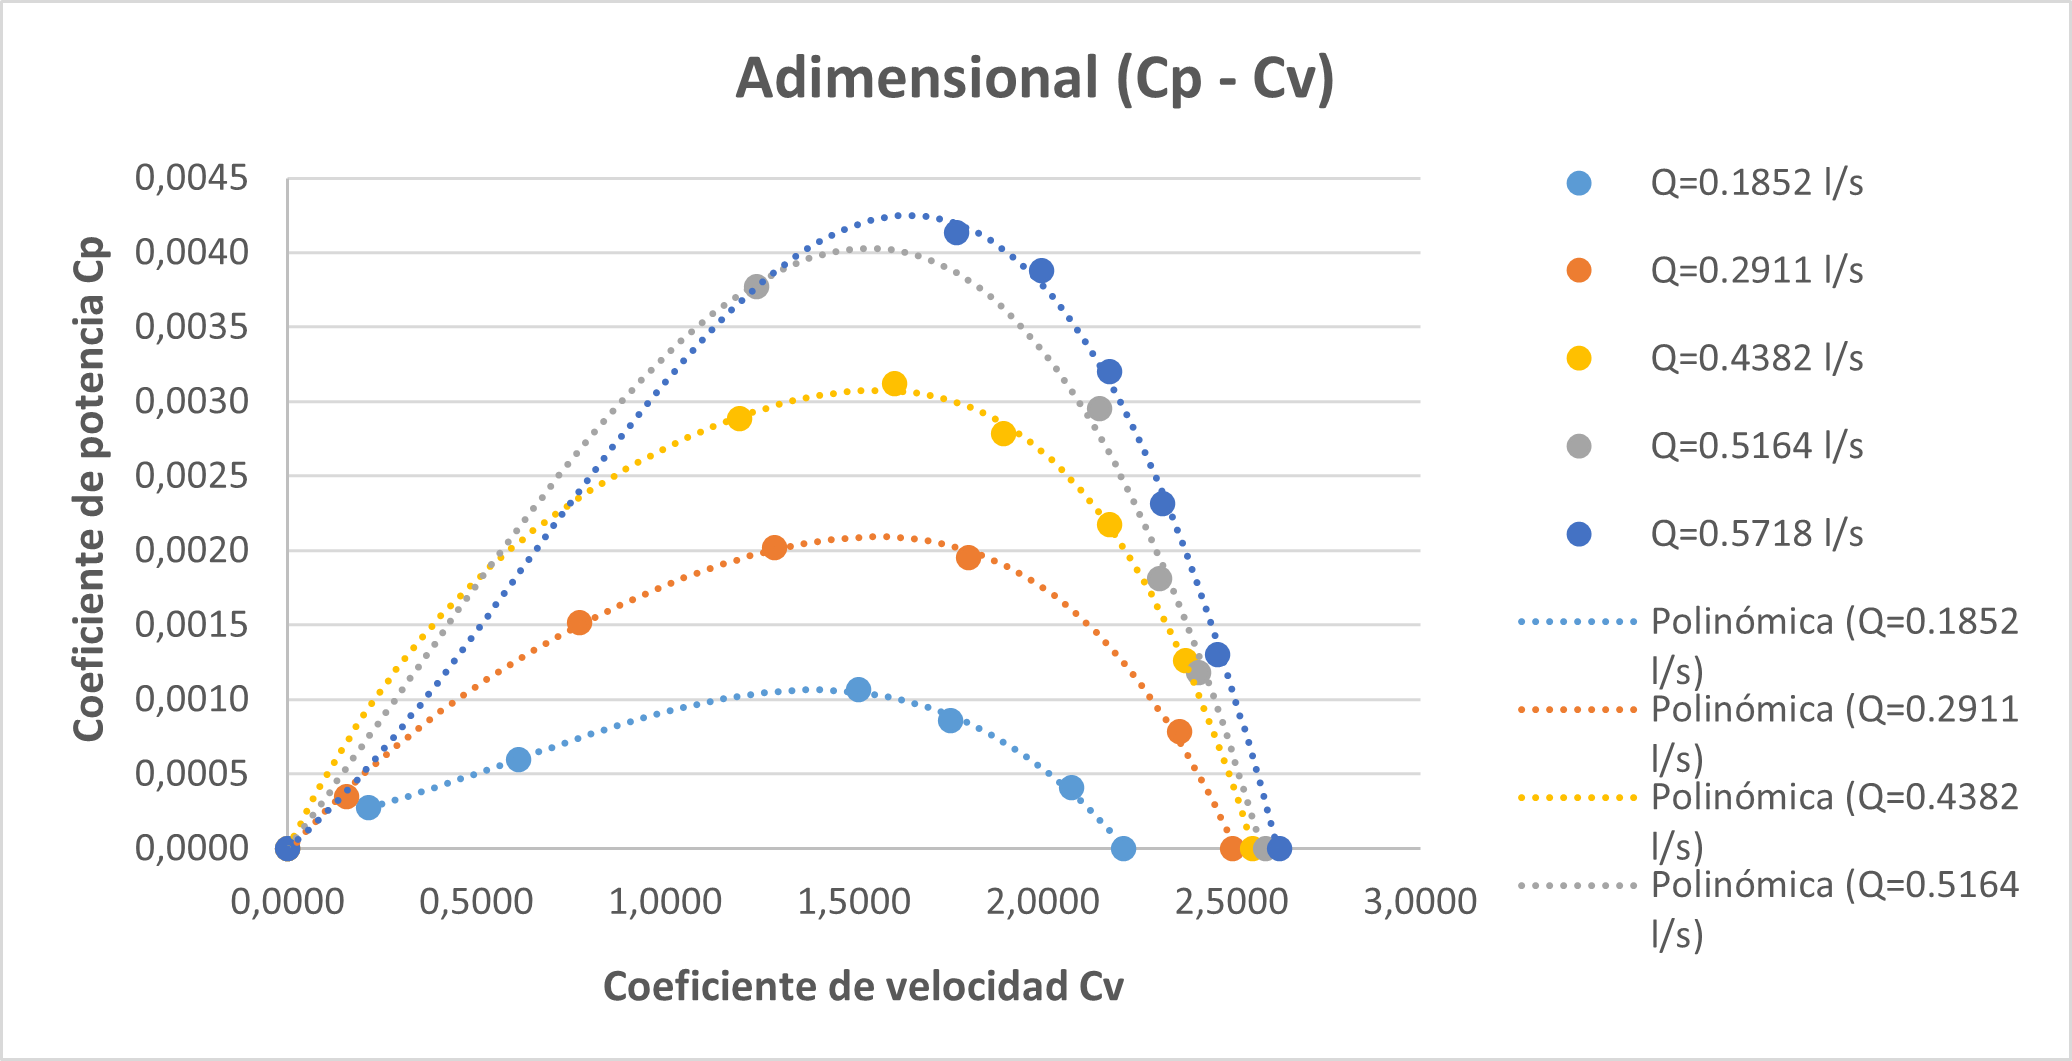
\includegraphics[width= 0.75 \textwidth]{Imagenes/Curvas de potencia frente a coeficiente de velocidad.png}
  \caption{Curvas de coeficiente de potencia ($C_p$) frente a coeficiente de velocidad ($C_v$)} 
  \label{fig: Curvas de coeficiente de potencia frente a coeficiente de velocidad}
\end{figure*}

A continuación, en la Fig. \ref{fig: Curvas de coeficiente de potencia frente a coeficiente de velocidad} se han representado los valores de coeficiente de potencia frente a los de coeficiente de velocidad obtenidos para cada uno de los 5 caudales, utilizando las expresiones (\ref{eq: Turbinas - Ecuacion 8}) y (\ref{eq: Turbinas - Ecuacion 9}). Estos coeficientes tienen carácter adimensional.

Antes de representar estas curvas en ejes adimensionales, lo que cabría esperar es la obtención de curvas semejantes a las representadas en la Fig. \ref{fig: Curvas de potencia frente a velocidad de giro}, ya que el único cambio que se ha llevado a cabo es la adimensionalización de las variables potencia y velocidad de giro.

Como se puede apreciar, se cumple la hipótesis previa planteada por el equipo teniendo en cuenta los conocimientos teóricos de la asignatura. Se obtienen finalmente curvas semejantes para todos los caudales.

En cuanto a los rangos, para el coeficiente de potencia se obtienen valores entre $0$ y $0.0045$. Esto es consecuencia de estar trabajando con una turbina de pequeñas dimensiones que desarrolla una potencia reducida. Por otro lado, se obtienen coeficientes de velocidad con valores entre $0$ y $3$.

Una vez representadas las curvas de potencia frente a velocidad de giro en ejes dimensionales y adimensionales, se procede análogamente con las curvas de rendimiento frente a velocidad de giro en ambos ejes.

El rendimiento se calcula mediante la expresión (\ref{eq: Turbinas - Ecuacion 6}). Al estar trabajando con una microturbina Pelton, se espera obtener un rendimiento máximo en el rango de 0.88 y 0.93, aunque al estar variando constantemente los caudales de trabajo y el par aplicado, se espera obtener un amplio rango de rendimientos.

\begin{figure*}[ht!]
  \centering
  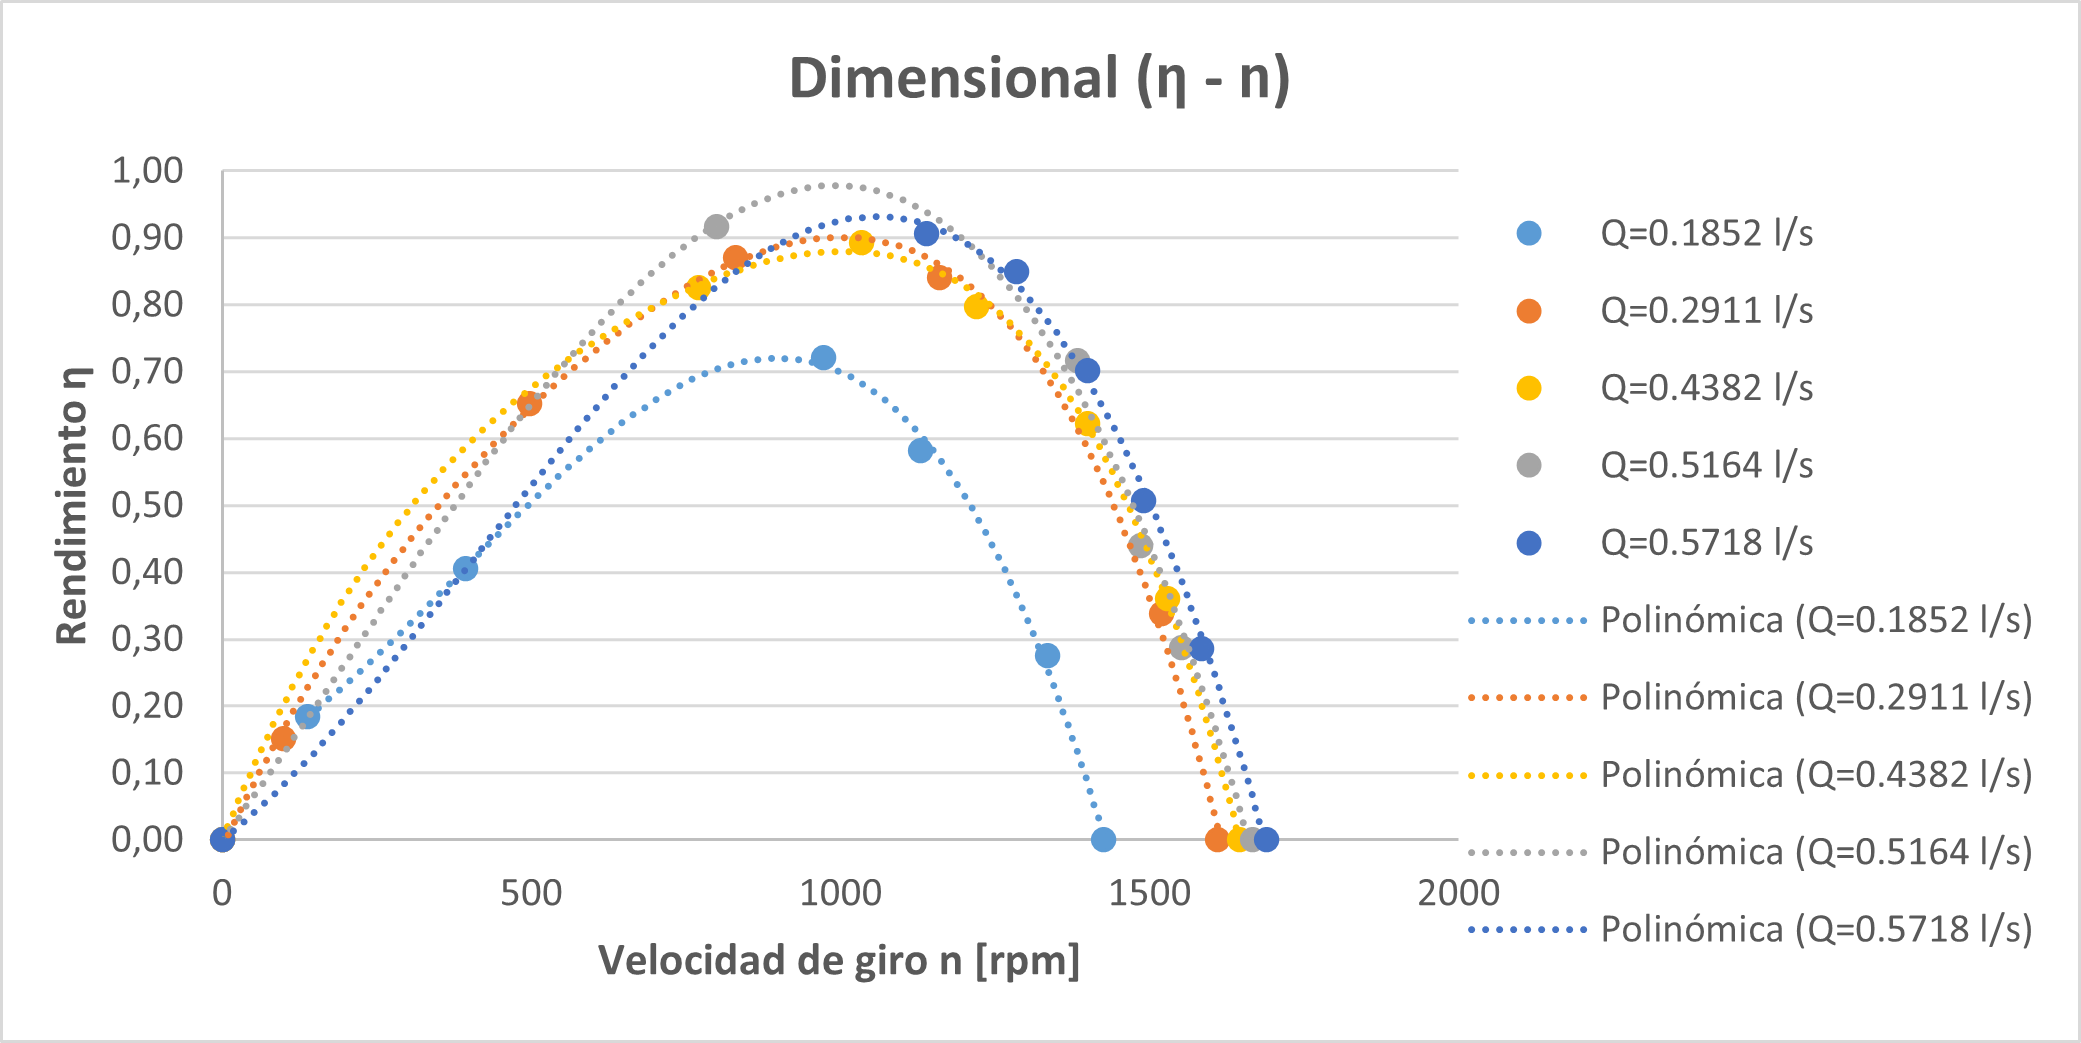
\includegraphics[width= 0.75 \textwidth]{Imagenes/Curvas de rendimiento frente a velocidad de giro.png}
  \caption{Curvas de rendimiento frente ($\eta$) a velocidad de giro ($n$)} 
  \label{fig: Curvas de rendimiento frente a velocidad de giro}
\end{figure*}

En la Fig. \ref{fig: Curvas de rendimiento frente a velocidad de giro} se representa el rendimiento frente a la velocidad de giro de la turbina para cada caudal tomado. Al igual que con la potencia, se espera que el rendimiento máximo para cada caudal se encuentre cerca de la mitad del valor máximo de régimen de giro de la turbina.

Como era de esperar, se cumple para todos los caudales. También se observa que, a mayor caudal, mayor rendimiento se puede alcanzar. Sin embargo, las curvas de rendimiento para los caudales mayores se encuentran mucho más cercanas que las de potencia. Esto puede ser consecuencia de que el caudal nominal con el que se obtiene el rendimiento óptimo no tiene por qué ser el máximo caudal alcanzado.

Los resultados obtenidos son satisfactorios, ya que se observa un comportamiento similar de todas las curvas, y se obtienen unos valores de rendimientos coherentes con la teoría. El valor de rendimiento máximo obtenido se puede obtener visualizando la Tabla \ref{tab: Medidas tomadas y valores relevantes para la representación de las curvas}. En este caso es $0.92$ y se da para un caudal de $0.516\ L/s$ y a una velocidad de giro de $799\ rpm$. Este valor de rendimiento máximo es consistente con el marco teórico.

\begin{figure*}[ht!]
  \centering
  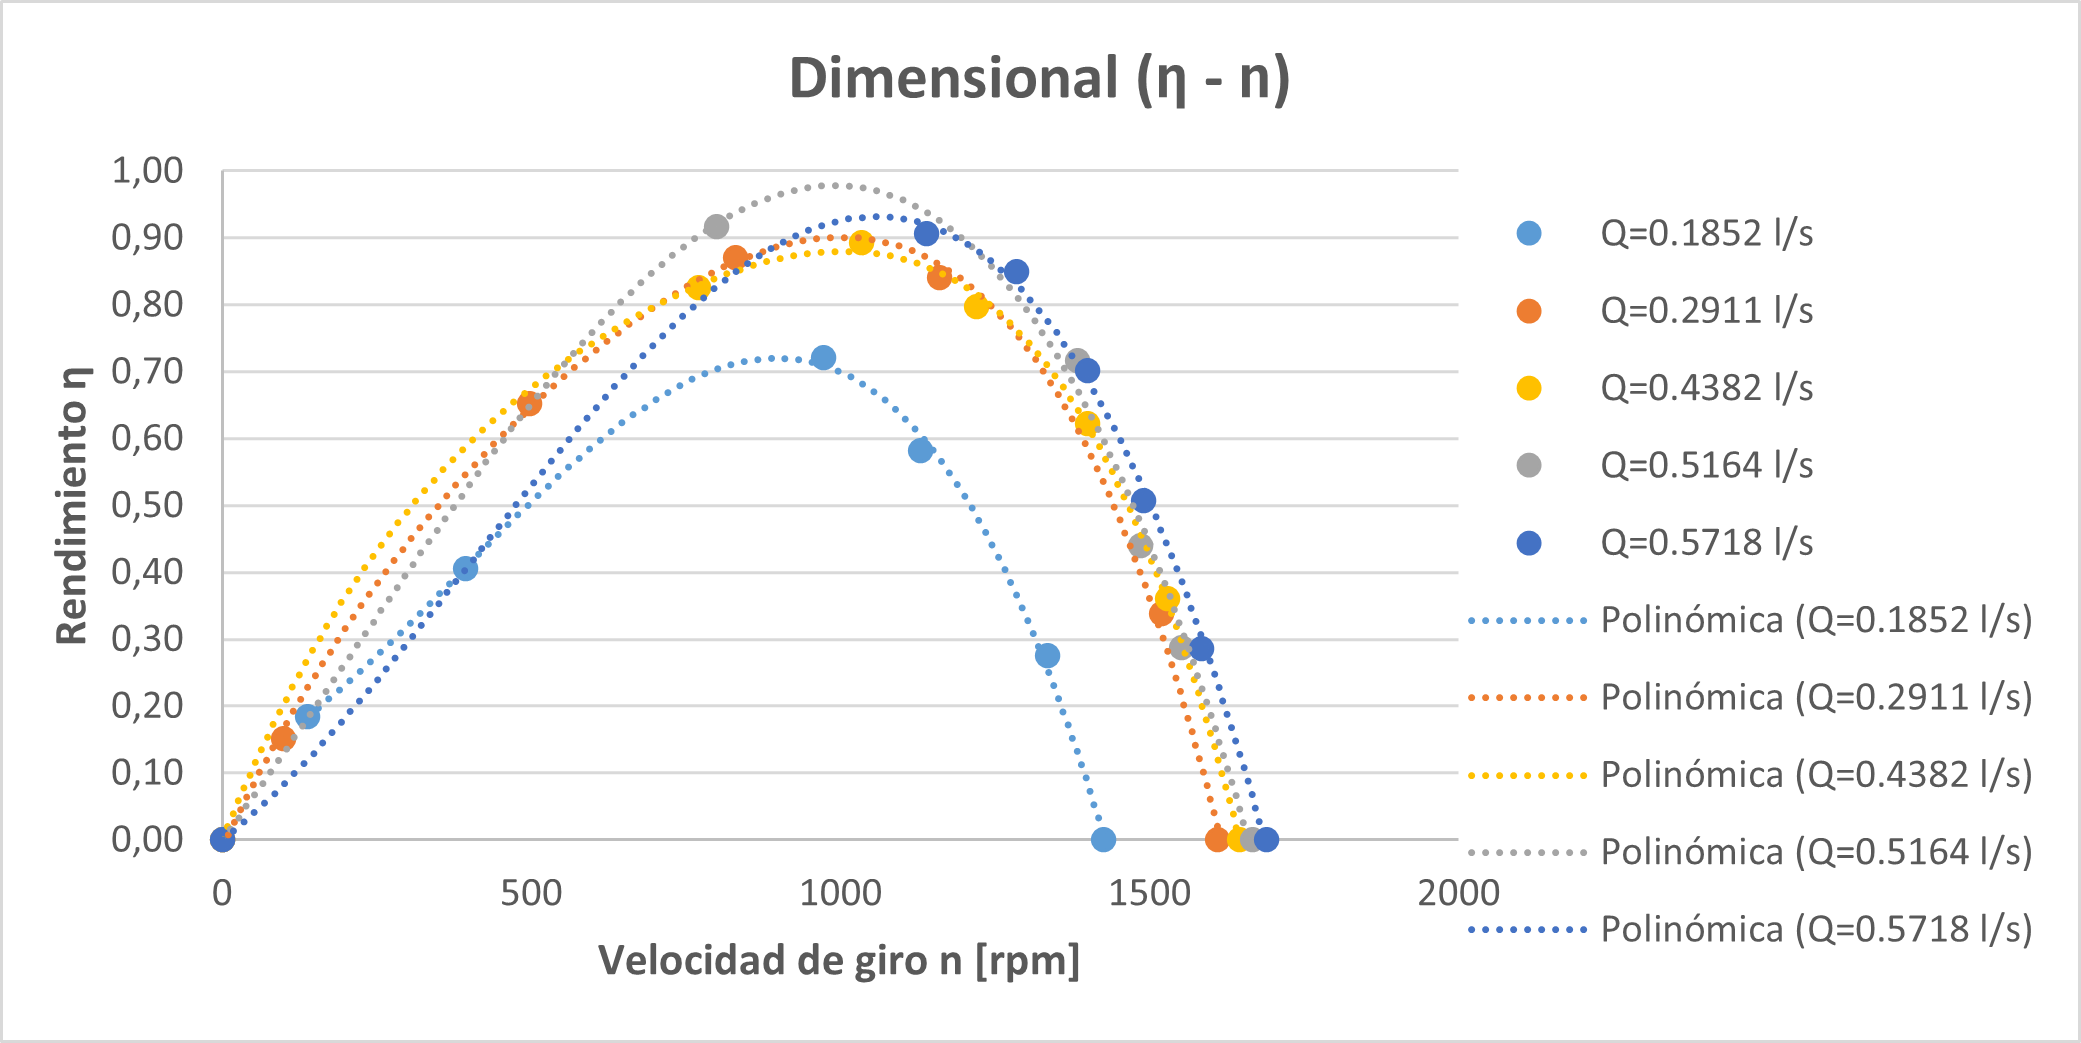
\includegraphics[width= 0.75 \textwidth]{Imagenes/Curvas de rendimiento frente a velocidad de giro.png}
  \caption{Curvas de rendimiento ($\eta$) frente a coeficiente de velocidad ($C_p$)} 
  \label{fig: Curvas de rendimiento frente a coeficiente de velocidad}
\end{figure*}

Por último, en la Fig. \ref{fig: Curvas de rendimiento frente a coeficiente de velocidad} se representan las curvas de rendimiento frente a velocidad en ejes adimensionales. Como puede comprobarse, las curvas son semejantes a las de rendimiento frente a velocidad de giro en ejes dimensionales de la Fig. \ref{fig: Curvas de rendimiento frente a velocidad de giro}. Esto denota un correcto uso de las ecuaciones para la realización de los cálculos.

Tanto en la Fig. \ref{fig: Curvas de rendimiento frente a velocidad de giro} como en la Fig. \ref{fig: Curvas de rendimiento frente a coeficiente de velocidad} se observa una tendencia creciente en las curvas de rendimiento a medida que va aumentando el régimen de giro. Esta tendencia se va frenando hasta alcanzar un máximo cerca del valor medio de la máxima velocidad de giro que puede dar la turbina. A continuación, la tendencia pasa a ser decreciente hasta llegar a 0, momento en el cual el rodete se ha frenado por completo al haber aplicado un par resistente muy grande.

Por lo tanto y a la vista de los resultados, se puede afirmar que la representación de las curvas pedidas es válida y se procede a obtener el resto de los resultados de interés.

Como se ha comentado anteriormente, el valor de rendimiento máximo obtenido por el equipo es $0.92$. Para este valor de rendimiento, se va a calcular la velocidad específica de la turbina ($\omega_s$). Este parámetro adimensional se utiliza para caracterizar el diseño de la turbina, y se obtiene adimensionalizando la velocidad angular $\omega$ mediante la siguiente expresión:
\begin{equation}
  \omega_s = \omega \frac{W_t^{1/2} \rho^{3/4}}{\Delta p^{5/4}}
  \label{eq: Turbinas - Ecuacion 11}
\end{equation}

A partir de la expresión (\ref{eq: Turbinas - Ecuacion 11}) y haciendo uso de las variables en condiciones de rendimiento máximo, se obtiene una velocidad específica de:
\[ \omega_s = 0.076 \]
\[ \eta_{max} = 0.92 \]

Según la teoría vista en clase, para una turbina Pelton la velocidad específica debe encontrarse entre $0.05$ y $0.35$, por lo que el valor de velocidad específica obtenido es acorde con la teoría de turbinas Pelton.

Además, se ha obtenido la velocidad específica para cada una de las medidas tomadas. Estos resultados se pueden observar en la Tabla \ref{tab: Medidas tomadas y valores relevantes para la representación de las curvas}. El rango de velocidades específicas obtenidas va desde un valor de $0.003$ hasta un valor de $0.124$. Al tratarse de una turbina Pelton de pequeñas dimensiones, este valor mínimo de velocidad específica puede ser coherente.

Cabe mencionar que los errores experimentales son más acusados en caudales altos, donde al llenarse el tanque más rápido, la medición del volumen se realiza de manera menos precisa.

\section{Conclusiones}
Tras haber realizado la práctica y haber obtenido todos los resultados pedidos, el equipo puede afirmar que la realización de esta práctica se ha llevado a cabo de manera satisfactoria.

Todos los integrantes del equipo han obtenido las mediciones exitosamente, y gracias a ello se ha podido disponer de datos para 5 caudales diferentes. Además, las mediciones se consiguieron realizar dentro del tiempo máximo permitido para obtener la nota más alta posible.

Por otra parte, los resultados obtenidos se asemejan mucho a lo esperado por el equipo de acuerdo con la teoría de turbinas hidráulicas, más concretamente de turbinas Pelton.

Para finalizar, es importante destacar todo lo aprendido a lo largo de la práctica, así como el valor que supone, para todo el equipo, la oportunidad de trabajar con maquinaria real. Este tipo de experiencias permite complementar la teoría con una aplicación práctica directa, favoreciendo una comprensión más completa y enriquecedora del funcionamiento de los sistemas estudiados.

\pagebreak
{\LARGE Aeroturbinas}
\setcounter{section}{0}
\setcounter{subsection}{0}
\setcounter{subsubsection}{0}

\section{Introducción}
\subsection{Objetivos de la práctica}
Esta práctica tiene como objetivo principal analizar el comportamiento de una aeroturbina de pequeño tamaño en condiciones controladas de laboratorio, mediante la determinación de su coeficiente de potencia $C_p$ y su velocidad específica $\lambda$. Ambos parámetros son adimensionales y permiten evaluar de forma general la eficiencia con la que la máquina convierte la energía del viento en potencia útil.

\subsection{Fundamentos teóricos}
Las turbomáquinas son dispositivos en los que se transfiere energía entre un fluido y un rotor, ya sea para generar trabajo o para consumirlo En el caso de las aeroturbinas, el fluido de trabajo es el aire, y el principio de funcionamiento se basa en la conversión de energía cinética y/o potencial del flujo en energía mecánica.

Uno de los aspectos clave en el análisis de turbinas es la triangulación de velocidades, que relaciona la velocidad absoluta del fluido ($V$), la velocidad relativa respecto al rotor ($W$) y la velocidad tangencial del rotor ($U$). Además, se estudia el coeficiente de carga y el rendimiento isentrópico, indicadores que permiten evaluar el desempeño del sistema.

En esta práctica se trabajó con una turbina axial, caracterizada por un flujo que mantiene una trayectoria aproximadamente paralela al eje del rotor. La regulación del ángulo de los álabes guía permite modificar el ángulo de entrada del flujo al rotor, lo que tiene un impacto directo en el rendimiento.

\section{Descripción del equipo de prácticas y metodología}

Para ello, se montó un sistema experimental compuesto por una aeroturbina con cuatro palas planas, un ventilador para simular el flujo de viento, un anemómetro para medir la velocidad del aire incidente, un potenciómetro que regula la carga eléctrica conectada al generador, y un tacómetro que permite conocer la velocidad angular del rotor. El equipo permite también la modificación del ángulo de paso $\beta$ de las palas, lo cual es fundamental en el control de la potencia generada.

Durante el desarrollo de la práctica se siguió un procedimiento iterativo que consistió en:
\begin{itemize}
  \item Fijar varias velocidades del viento distintas, medidas con un anemómetro.
  \item Para cada velocidad, se seleccionaron varios valores del ángulo de paso $\beta$ (0°, 22.5°, 45°, 67.5° y 90°).
  \item A continuación, se variaba la carga de resistencia conectada al generador mediante el potenciómetro, lo cual alteraba la velocidad de giro del rotor.
  \item Para cada combinación de parámetros, se midieron los valores de tensión, intensidad y velocidad angular, a partir de los cuales se calcularon la potencia eléctrica generada $W$, el coeficiente de potencia $C_p$, y la velocidad específica $\lambda$.
\end{itemize}

Con los datos recopilados, se construyeron las curvas $C_p - \lambda$, fundamentales para evaluar el comportamiento de la aeroturbina bajo diferentes condiciones de operación. Además, se analizaron casos límite como los ángulos de paso $\beta$ = 0° y $\beta$ = 90°, para interpretar su efecto sobre la producción de potencia. Finalmente, se compararon los resultados experimentales con los comportamientos teóricos esperados, detectando posibles discrepancias y causas.

\section{Resultados}
En esta sección se presentan los resultados experimentales obtenidos durante la práctica. Se ha completado una tabla con los valores medidos y calculados para cada combinación de velocidad del viento, ángulo de paso y resistencia eléctrica. A partir de estos datos, se ha determinado la potencia generada, la velocidad angular del rotor y los coeficientes adimensionales $C_p$ y $\lambda$ para cada caso analizado.

En el ensayo se tomaron medidas para los ángulos 0º, 22.5º, 45º, 67.5º y 90º, cuyos resultados así como los cálculos pedidos, se muestran en la tabla \ref{tab: Aeroturbinas}.

\begin{table*}[ht!]
  \centering
  \caption{Resultados experimentales: Cp y $\lambda$ para distintos valores de $\beta$}
  \label{tab: Aeroturbinas}
  \begin{tabular}{|c|c|c|c|c|c|c|c|}
    \hline
    $\beta$ [º] & $v$ [m/s] & $I$ [mA] & $U$ [V] & $\omega$ [rad/s] & $W$ [W] & $C_P$ & $\lambda$ \\
    \hline
    \multirow{6}{*}{0} & 7.5 & 1 & 0.02 & 6.98 & 0.00002 & 0.000007 & 31.41 \\
    \cline{2-8}
    & 10 & 4.8 & 0.15 & 12.566 & 0.00072 & 0.000106 & 42.412 \\
    \cline{2-8}
    & 10 & 3.7 & 0.18 & 11.17 & 0.000666 & 0.000098 & 37.699 \\
    \cline{2-8}
    & 10 & 3 & 0.19 & 12.566 & 0.00057 & 0.000084 & 42.412 \\
    \cline{2-8}
    & 10 & 2.2 & 0.2 & 13.963 & 0.00044 & 0.000065 & 47.124 \\
    \cline{2-8}
    & 10 & 1.9 & 0.21 & 15.359 & 0.000399 & 0.000059 & 51.836 \\
    \hline
    \multirow{11}{*}{22.5} & 7 & 1.5 & 0.06 & 6.283 & 0.00009 & 0.000039 & 30.294 \\
    \cline{2-8}
    & 7 & 1.1 & 0.05 & 5.585 & 0.000055 & 0.000024 & 26.928 \\
    \cline{2-8}
    & 7 & 0.7 & 0.05 & 3.491 & 0.000035 & 0.000015 & 16.83 \\
    \cline{2-8}
    & 7 & 0.7 & 0.07 & 4.887 & 0.000049 & 0.000021 & 23.562 \\
    \cline{2-8}
    & 7 & 0.4 & 0.05 & 3.491 & 0.00002 & 0.000009 & 16.83 \\
    \cline{2-8}
    & 7.5 & 9.2 & 0.55 & 43.28 & 0.00506 & 0.001761 & 194.76 \\
    \cline{2-8}
    & 10 & 23.8 & 0.6 & 58.643 & 0.01428 & 0.002096 & 197.921 \\
    \cline{2-8}
    & 10 & 15.3 & 0.75 & 59.341 & 0.011475 & 0.001684 & 200.277 \\
    \cline{2-8}
    & 10 & 11.6 & 0.79 & 60.039 & 0.009164 & 0.001345 & 202.633 \\
    \cline{2-8}
    & 10 & 9.2 & 0.81 & 61.436 & 0.007452 & 0.001094 & 207.346 \\
    \cline{2-8}
    & 10 & 7.7 & 0.83 & 64.228 & 0.006391 & 0.000938 & 216.77 \\
    \hline
    \multirow{13}{*}{45} & 6 & 6.9 & 0.7 & 54.454 & 0.00483 & 0.003282 & 306.305 \\
    \cline{2-8}
    & 7 & 10.3 & 1.03 & 78.19 & 0.010609 & 0.00454 & 376.988 \\
    \cline{2-8}
    & 7 & 12.3 & 0.98 & 78.19 & 0.012054 & 0.005159 & 376.988 \\
    \cline{2-8}
    & 7 & 16.9 & 0.85 & 71.9 & 0.014365 & 0.006148 & 346.661 \\
    \cline{2-8}
    & 7 & 25.5 & 0.62 & 62.83 & 0.01581 & 0.006766 & 302.93 \\
    \cline{2-8}
    & 7.5 & 23.1 & 0.52 & 53.06 & 0.012012 & 0.00418 & 238.77 \\
    \cline{2-8}
    & 9 & 22 & 1.12 & 92.85 & 0.02464 & 0.004962 & 348.188 \\
    \cline{2-8}
    & 9 & 13 & 1.28 & 101.93 & 0.01664 & 0.003351 & 382.238 \\
    \cline{2-8}
    & 10 & 45.8 & 1.2 & 117.985 & 0.05496 & 0.008068 & 398.198 \\
    \cline{2-8}
    & 10 & 30.7 & 1.45 & 130.551 & 0.044515 & 0.006535 & 440.609 \\
    \cline{2-8}
    & 10 & 23.2 & 1.6 & 131.249 & 0.03712 & 0.005449 & 442.966 \\
    \cline{2-8}
    & 10 & 19 & 1.65 & 134.042 & 0.03135 & 0.004602 & 452.39 \\
    \cline{2-8}
    & 10 & 15.5 & 1.72 & 139.627 & 0.02666 & 0.003914 & 471.24 \\
    \hline
    \multirow{14}{*}{67.5} & 7 & 24 & 1 & 78.191 & 0.024 & 0.010271 & 376.992 \\
    \cline{2-8}
    & 7 & 21 & 1.16 & 92.154 & 0.02436 & 0.010425 & 444.312 \\
    \cline{2-8}
    & 7 & 16.3 & 1.27 & 100.531 & 0.020701 & 0.008859 & 484.704 \\
    \cline{2-8}
    & 7 & 14 & 1.36 & 109.607 & 0.01904 & 0.008149 & 528.462 \\
    \cline{2-8}
    & 7 & 12.6 & 1.4 & 113.796 & 0.01764 & 0.007549 & 548.658 \\
    \cline{2-8}
    & 7.5 & 23.2 & 1.58 & 129.15 & 0.036656 & 0.012755 & 581.175 \\
    \cline{2-8}
    & 10 & 66.2 & 1.78 & 174.533 & 0.117836 & 0.017298 & 589.05 \\
    \cline{2-8}
    & 10 & 48.4 & 2.3 & 202.459 & 0.11132 & 0.016341 & 683.298 \\
    \cline{2-8}
    & 10 & 37.4 & 2.6 & 214.327 & 0.09724 & 0.014274 & 723.353 \\
    \cline{2-8}
    & 10 & 30.3 & 2.8 & 216.421 & 0.08484 & 0.012454 & 730.422 \\
    \cline{2-8}
    & 10 & 26.2 & 2.85 & 221.308 & 0.07467 & 0.010961 & 746.915 \\
    \cline{2-8}
    & 6 & 24.24 & 0.18 & 29.322 & 24.24 & 0.002965 & 0.291 \\
    \cline{2-8}
    & 6 & 20 & 0.52 & 48.869 & 20 & 0.007068 & 0.485 \\
    \cline{2-8}
    & 6 & 17 & 0.8 & 69.813 & 17 & 0.000243 & 0.692 \\
    \hline
    \multirow{1}{*}{90} & 7.5 & 0 & 0 & 0 & 0 & 0 & 0 \\
    \hline
  \end{tabular}
\end{table*}

\subsection{Representación de curvas $C_p - \lambda$}

\begin{figure*}[ht!]
  \centering
  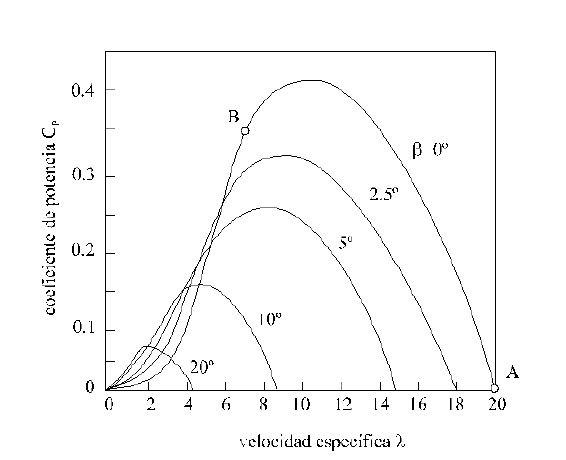
\includegraphics[width= 0.75 \textwidth]{Imagenes/Aeroturbinas Figura 3.1.jpg}
  \caption{Curvas teóricas del coeficiente de potencia $C_p$ en función de la velocidad específica $\lambda$ para distintos ángulos de paso}
  \label{fig: Aeroturbinas - Figura 3.1 guion}
\end{figure*}

A continuación, se representan gráficamente las curvas del coeficiente de potencia $C_p$ en función de la velocidad específica $\lambda$ para distintos valores del ángulo de paso $\beta$. Estas curvas permiten evaluar el comportamiento de la aeroturbina y comprobar si se cumplen las tendencias teóricas esperadas, tal como se describe en la Figura \ref{fig: Aeroturbinas - Figura 3.1 guion} del guion. Cada curva ha sido obtenida agrupando los datos experimentales correspondientes a un mismo valor de $\beta$ y distintas condiciones de velocidad del viento.

\begin{figure*}[ht!]
  \centering
  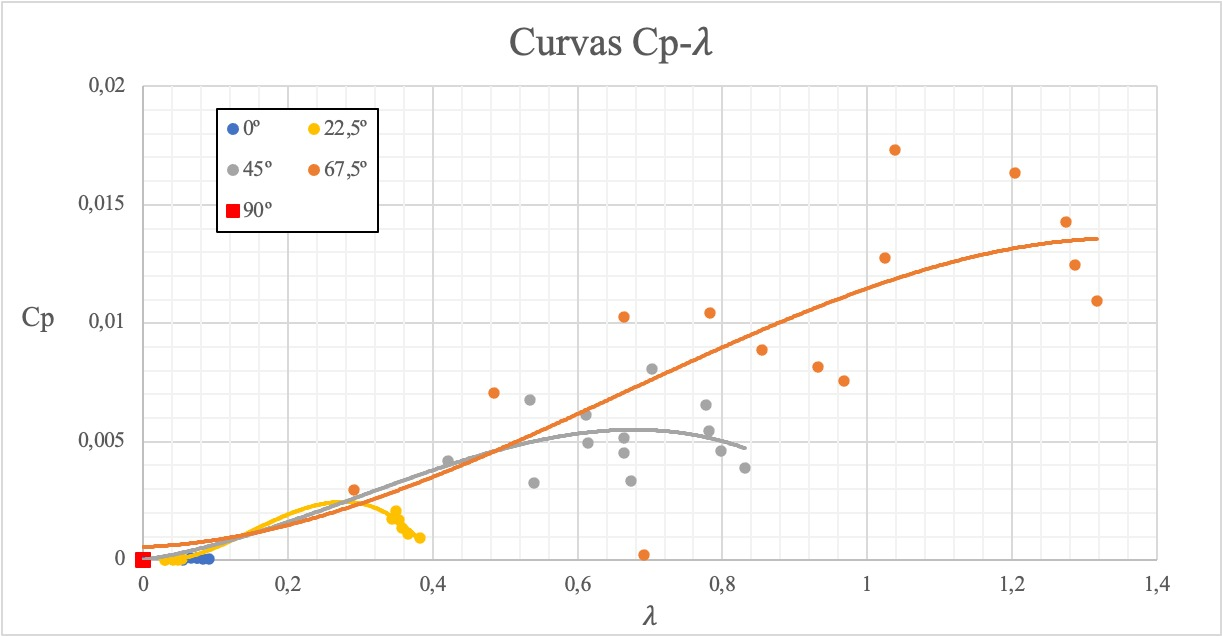
\includegraphics[width= 0.75 \textwidth]{Imagenes/Aeroturbinas Figura 1.jpg}
  \caption{Curva experimental de $C_p$ vs $\lambda$}
  \label{fig: Aeroturbinas - Figura 1}
\end{figure*}

\subsection{Comentar el comportamiento para los ángulos de paso $\beta$ = 0º y $\beta$ = 90º}

En primer lugar, es necesario definir cuál es el ángulo $\beta$, durante la práctica realizada nos referimos a este cómo el complementario al ángulo de calado $\theta$ definido entre la cuerda del perfil y el plano de giro del rotor.

En la práctica con palas planas, no se tomaron datos para el caso $\beta$ = 90°, ya que, como se observó en el laboratorio, al colocar las palas con este ángulo, la aeroturbina no presentaba movimiento alguno. Esto se debe a que, en esa posición, las palas se encuentran completamente perpendiculares al flujo del viento, actuando como una pared que impide el paso del aire. En consecuencia, no se genera par sobre el rotor, ni se producen tensión o corriente, lo que imposibilita calcular el coeficiente de potencia $C_p$.

En cuanto al caso $\beta$ = 0°, al inicio de la práctica se realizó una prueba colocando las palas en esta posición con la intención de que, al encender el ventilador, el aerogenerador permaneciera inmóvil. Teóricamente, al colocar las palas de forma perfectamente simétrica y con $\beta$ = 0°, no debería generarse ningún movimiento en la aeroturbina.

Sin embargo, tras dos intentos, se observó que si giraba. Esto se puede deber a imprecisiones en la fabricación de las palas o en su posicionamiento, que impidieron una simetría perfecta. Como puede apreciarse en los resultados obtenidos con este ángulo ($\beta$ = 0°), los valores de tensión e intensidad que se obtuvieron fueron significativamente más bajos, lo que se traduce en un coeficiente de potencia $C_p$ también reducido.

\subsection{Analizar si se cumplen las tendencias esperadas, de acuerdo con la figura \ref{fig: Aeroturbinas - Figura 3.1 guion}, y razonar las posibles discrepancias.}

Al comparar las curvas obtenidas experimentalmente con las curvas teóricas de la Figura \ref{fig: Aeroturbinas - Figura 3.1 guion}, se observa que, en términos generales, ambas presentan una tendencia creciente del coeficiente de potencia $C_p$ respecto a la velocidad específica $\lambda$, al menos en los primeros tramos. Sin embargo, existen discrepancias importantes tanto en la forma como en los valores máximos alcanzados.

En la gráfica teórica, el coeficiente de potencia $C_p$ alcanza valores de hasta 0.42 para un ángulo de paso $\beta$=0º, disminuyendo progresivamente a medida que aumenta el ángulo. Este comportamiento no se reproduce 3en los datos experimentales, donde el $C_p$ máximo apenas alcanza 0.015 y las diferencias entre las curvas correspondientes a distintos ángulos de paso son mínimas. Mientras que en la Figura \ref{fig: Aeroturbinas - Figura 1} el coeficiente de potencia aumenta al disminuir el ángulo de paso $\beta$, en los resultados experimentales del laboratorio se observa la tendencia opuesta.

Estas discrepancias pueden explicarse por efectos de escala (uso de modelos pequeños), pérdidas por fricción, errores de medición. También es posible que la interacción entre el viento y las palas no haya sido óptima debido a las dimensiones reducidas del sistema experimental, lo que limita la eficiencia real y, por tanto, los valores de $C_p$.

En conclusión, aunque las curvas experimentales muestran una tendencia general creciente de $C_p$ con $\lambda$, no reproducen con fidelidad los valores ni la forma de las curvas teóricas.

\section{Conclusiones}
Aunque durante la práctica no se tomaron datos experimentales con distinto número de palas ni con perfiles curvados, es posible extraer conclusiones relevantes basadas en la teoría del guion y en la experiencia obtenida con las palas planas.

En primer lugar, respecto al número de palas, se sabe que este influye en el comportamiento aerodinámico de la turbina. Menos palas reducen la resistencia y permiten mayores velocidades específicas $\lambda$, aunque dificultan el arranque a bajas velocidades. Más palas, en cambio, facilitan el arranque pero generan más fricción, reduciendo la eficiencia a altas revoluciones. En esta práctica se emplearon cuatro palas planas, una configuración equilibrada entre par de arranque y rendimiento moderado.

En cuanto al perfil aerodinámico, el uso de palas planas simplifica el montaje pero no es óptimo en términos de eficiencia. Los perfiles curvados están diseñados para maximizar la sustentación y mejorar la interacción con el flujo de aire, permitiendo obtener valores más altos del coeficiente de potencia $C_p$. Los valores máximos de $C_p$ medidos en el ensayo (alrededor de 0.017) son notablemente inferiores a los teóricos ($\approx$ 0.4), lo que indica que la geometría y el diseño de las palas tienen un papel clave en el rendimiento global de la máquina.

Por tanto, aunque esta práctica se centró en el estudio del ángulo de paso, los resultados muestran que para mejorar el aprovechamiento de la energía eólica sería necesario optimizar también tanto el número de palas como su perfil. Estos factores, junto con un control adecuado del ángulo $\beta$, permiten maximizar la eficiencia de la turbina y acercarse a los valores ideales previstos por la teoría.

Respecto al ángulo de paso de las palas, se ha comprobado a lo largo del ensayo que tiene un efecto determinante sobre el comportamiento de la turbinas. Para ángulos bajos, el rotor logra girar y generar potencia, aunque en valores muy reducidos. En cambio, en el caso extremo de $\beta$=90º, la aeroturbina deja de girar por completo, actuando las palas como una superficie perpendicular que bloquea el flujo del viento.

Por último, las diferencias entre los resultados de $C_p$ obtenidos y los teóricos pueden atribuirse a varios factores, como el uso de un modelo a escala, pérdidas por fricción, turbulencias no controladas y un diseño de palas no optimizado. Asimismo, las curvas $C_p - \lambda$ obtenidas muestran una tendencia creciente en los primeros tramos, pero no reproducen con precisión la forma ni los máximos esperados.

Pese a estas limitaciones, la práctica ha sido útil para visualizar de manera clara los efectos de los distintos parámetros sobre el comportamiento de la aeroturbina.

\end{document}